%----------
%   WARNING
%----------

% This Guide contains Library recommendations based mainly on APA and IEEE styles, but you must always follow the guidelines of your TFG Tutor and the TFG regulations for your degree.

% THIS TEMPLATE IS BASED ON THE APA STYLE 


%----------
% DOCUMENT SETTINGS
%----------

\documentclass[12pt]{report} % font: 12pt

% margins: 2.5 cm top and bottom; 3 cm left and right
\usepackage[
a4paper,
vmargin=2.5cm,
hmargin=3cm
]{geometry}

% Paragraph Spacing and Line Spacing: Narrow (6 pt / 1.15 spacing) or Moderate (6 pt / 1.5 spacing)
\renewcommand{\baselinestretch}{1.15}
\parskip=6pt

% Color settings for cover and code listings 
\usepackage[table]{xcolor}
\definecolor{azulUC3M}{RGB}{0,0,102}
\definecolor{gray97}{gray}{.97}
\definecolor{gray75}{gray}{.75}
\definecolor{gray45}{gray}{.45}

% In the template we include the file OUTPUT.XMPDATA. You can download that file and include the metadata that will be incorporated into the PDF file when you compile the memoria.tex file. Then upload it back to your project. 
% Commented out due to upstream error
% \use package[a-1b]{pdf}

% LINKS
\usepackage{hyperref}
\hypersetup{colorlinks=true,
	linkcolor=black, % links to parts of the document (e.g. index) in black
	urlcolor=blue} % links to resources outside the document in blue

% MATH EXPRESSIONS
\usepackage{amsmath,amssymb,amsfonts,amsthm}

% Character encoding
\usepackage{txfonts} 
\usepackage[T1]{fontenc}
\usepackage[utf8]{inputenc}

% English settings
\usepackage[spanish]{babel} 
\usepackage[babel, spanish=spanish]{csquotes}
\AtBeginEnvironment{quote}{\small}

% Footer settings
\usepackage{fancyhdr}
\pagestyle{fancy}
\fancyhf{}
\renewcommand{\headrulewidth}{0pt}
\rfoot{\thepage}
\fancypagestyle{plain}{\pagestyle{fancy}}

% DESIGN OF THE TITLES of the parts of the work (chapters and epigraphs or sub-chapters)
\usepackage{titlesec}
\usepackage{titletoc}
\titleformat{\chapter}[block]
{\large\bfseries\filcenter}
{\thechapter.}
{5pt}
{\MakeUppercase}
{}
\titlespacing{\chapter}{0pt}{0pt}{*3}
\titlecontents{chapter}
[0pt]                                               
{}
{\contentsmargin{0pt}\thecontentslabel.\enspace\uppercase}
{\contentsmargin{0pt}\uppercase}                        
{\titlerule*[.7pc]{.}\contentspage}                 

\titleformat{\section}
{\bfseries}
{\thesection.}
{5pt}
{}
\titlecontents{section}
[5pt]                                               
{}
{\contentsmargin{0pt}\thecontentslabel.\enspace}
{\contentsmargin{0pt}}
{\titlerule*[.7pc]{.}\contentspage}

\titleformat{\subsection}
{\normalsize\bfseries}
{\thesubsection.}
{5pt}
{}
\titlecontents{subsection}
[10pt]                                               
{}
{\contentsmargin{0pt}                          
	\thecontentslabel.\enspace}
{\contentsmargin{0pt}}                        
{\titlerule*[.7pc]{.}\contentspage}  


% Tables and figures settings
\usepackage{multirow} % combine cells 
\usepackage{caption} % customize the title of tables and figures
\usepackage{floatrow} % we use this package and its \ ttabbox and \ ffigbox macros to align the table and figure names according to the defined style.
\usepackage{array} % with this package we can define in the following line a new type of column for tables: custom width and centered content
\newcolumntype{P}[1]{>{\centering\arraybackslash}p{#1}}
\DeclareCaptionFormat{upper}{#1#2\uppercase{#3}\par}
\usepackage{graphicx}
\graphicspath{{../imagenes/}} % images folder

% Table layout for social sciences and humanities
\captionsetup*[table]{
	justification=raggedright,
	labelsep=newline,
	labelfont=small,
	singlelinecheck=false,
	labelfont=bf,
	font=small,
	textfont=it
}

% Figure layout for social sciences and humanities
\captionsetup[figure]{
	%name=Figura,
	singlelinecheck=off,
	labelsep=newline,
	font=small,
	labelfont=bf,
	textfont=it
}
\floatsetup[figure]{
    style=plaintop,
    heightadjust=caption,
    footposition=bottom,
    font=small
}

% Figures and tables footnote layout 
\captionsetup*[floatfoot]{
    footfont={small, up}
}

% FOOTNOTES
\usepackage{chngcntr} % continuous numbering of footnotes
\counterwithout{footnote}{chapter}

% CODE LISTINGS 
% support and styling for listings. More information in  https://es.wikibooks.org/wiki/Manual_de_LaTeX/Listados_de_código/Listados_con_listings
\usepackage{listings}

% Custom listing
\lstdefinestyle{estilo}{ frame=Ltb,
	framerule=0pt,
	aboveskip=0.5cm,
	framextopmargin=3pt,
	framexbottommargin=3pt,
	framexleftmargin=0.4cm,
	framesep=0pt,
	rulesep=.4pt,
	backgroundcolor=\color{gray97},
	rulesepcolor=\color{black},
	%
	basicstyle=\ttfamily\footnotesize,
	keywordstyle=\bfseries,
	stringstyle=\ttfamily,
	showstringspaces = false,
	commentstyle=\color{gray45},     
	%
	numbers=left,
	numbersep=15pt,
	numberstyle=\tiny,
	numberfirstline = false,
	breaklines=true,
	xleftmargin=\parindent
}

\captionsetup*[lstlisting]{font=small, labelsep=period}
 
\lstset{style=estilo}
\renewcommand{\lstlistingname}{\uppercase{Código}}


% REFERENCES 

\usepackage{color}

% used for cite command, and changing the color the URL and dates are.
\usepackage{hyperref} 
\hypersetup{
    colorlinks=true,
    linkcolor=blue,
    urlcolor=blue,
    linktoc=all,
    citecolor=black
           }

% APA bibliography setup
\usepackage[style=apa, backend=biber, natbib=true, hyperref=true, uniquelist=false, sortcites]{biblatex}

\addbibresource{referencias.bib} % The references.bib file in which the bibliography used should be

% Caption package, for use of subfigures.
\usepackage{subfig}

% Create a list of glossaries and acronyms
\usepackage[acronym]{glossaries}
\makeglossaries



%Declare a new custom dash command
\DeclareRobustCommand\dash{ \unskip\nobreak\thinspace\textemdash\thinspace\ignorespaces}

%-------------
%	DOCUMENT
%-------------

\begin{document}

\pagenumbering{roman} % Roman numerals are used in the numbering of the pages preceding the body of the work.
	
%----------
%	COVER
%----------	
\begin{titlepage}
	\begin{sffamily}
  \begin{figure}%
    \raggedleft
    \subfloat{{
\includegraphics[width=3cm]{UNED.jpg} }}%
    \hspace*{\fill}
    \subfloat{{
\includegraphics[width=5cm]{Scalefast.jpg} }}%
\end{figure}
	\begin{center}
		\vspace{2.5cm}
		\begin{Large}
			Master en Ciberseguridad\\			
			 2020-2021\\
			\vspace{2cm}		
			\textsl{Trabajo de final de Master}
			\bigskip
			
		\end{Large}
		 	{\Huge ``Definicion, creacion e implementaicon del SecDevOps''}\\
		 	\vspace*{0.5cm}
	 		\rule{10.5cm}{0.1mm}\\
			\vspace*{0.9cm}
			{\LARGE Sergio Rosello Morell}\\ 
			\vspace*{1cm}
		\begin{Large}
			David Aracil Cofrade\\
			Rafael Pastor Vargas\\
			Madrid, a \today \\
		\end{Large}
	\end{center}
	\vfill
	\color{black}
	\fbox{
	\begin{minipage}{\linewidth}
    	\textbf{AVOID PLAGIARISM}\\
    	\footnotesize{The University uses the \textbf{Turnitin Feedback Studio} for the delivery of student work. This program compares the originality of the work delivered by each student with millions of electronic resources and detects those parts of the text that are copied and pasted. Plagiarizing in a TFM is considered a  \textbf{\underline{Serious Misconduct}}, and may result in permanent expulsion from the University.}\end{minipage}}

	% IF OUR WORK IS TO BE PUBLISHED UNDER A CREATIVE COMMONS LICENSE, INCLUDE THESE LINES. IS THE RECOMMENDED OPTION.
	\noindent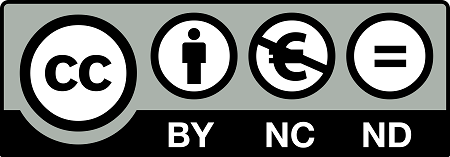
\includegraphics[width=4.2cm]{creativecommons.png}\\ % Creative Commons Logo
    \footnotesize{This work is licensed under Creative Commons \textbf{Attribution – Non Commercial – Non Derivatives}}
	
	\end{sffamily}
\end{titlepage}

\newpage % blank page
\thispagestyle{empty}
\mbox{}




%----------
%	ABSTRACT AND KEYWORDS 
%----------	
\renewcommand\abstractname{\large\bfseries\filcenter\uppercase{Sumario}}
\begin{abstract}
\thispagestyle{plain}
\setcounter{page}{3}
	
Inicio del movimiento DevOps, el 2010, con el desarrollo agil\\
Adopcion de la cultura agil por silicon valley y resto de munto\\
Implementacion de seguridad dentro del desarrollo agil\\
Uso de Pipelines, para desarrollar SW con la seguridad en mente\\
Caso especifico de la implementacion en Scalefast\\
\vfill
\end{abstract}
	
\newpage % Blank page
\renewcommand\abstractname{\large\bfseries\filcenter\uppercase{Abstract}}
\begin{abstract}
\thispagestyle{plain}
\setcounter{page}{5}

Start of Agile SW development, and DevOps culture\\
Adoption of culture by Silicon Valley and subsequent popularization\\
Security inside agile development?\\
Use of Pipelines in security-focused Agile development\\
Specific case with Scalefast\\

\textbf{Palabras clave:} % add the keywords
	
\vfill
\end{abstract}
\newpage % Blank page
\thispagestyle{empty}
\mbox{}


%----------
%	Dedication
%----------	
\chapter*{Agradecimientos}

\setcounter{page}{7}
	
Agradecer principalmente este trabajo a:

\begin{itemize}
  \item{Familia}
  \item{Tutores}
  \item{UNED}
  \item{Scalefast}
\end{itemize}

		
	\vfill
	
	\newpage % blank page
	\thispagestyle{empty}
	\mbox{}
	




%----------
%	TOC
%----------	

%--
% TOC
%-
\tableofcontents
\thispagestyle{fancy}

\newpage % blank page
\thispagestyle{empty}
\mbox{}




%--
% List of figures. If they are not included, comment the following lines
%-
\listoffigures
\thispagestyle{fancy}

\newpage % blank page
\thispagestyle{empty}
\mbox{}




%--
% List of tables. If they are not included, comment the following lines
%-
\listoftables
\thispagestyle{fancy}

\newpage % blankpage
\thispagestyle{empty}
\mbox{}





\newglossaryentry{job}
{
        name=job,
        description={Proceso ejecutado automáticamente, a partir de un evento externo, varios jobs ordenados de forma lógica forman un pipeline}
}
\newglossaryentry{API}
{
        name=Application Programming Interface, description={Permite que un
        servicio y un producto se comuniquen, permitiendo al producto crear una
        funcionalidad usando la información que proporciona el servicio a través
        de una interfaz estipulada.  Los desarrolladores no necesitan saber como
        se ha implementado el servicio, solamente, como se usa, para obtener la
        información requerida.}
}
\newglossaryentry{staging}
{
        name=staging,
        description={Un entorno que reproduce exactamente el entorno de producción cuya finalidad es asegurar que el código que se va a desplegar en producción funcione correctamente}
}
\newglossaryentry{App-Sec}
{
        name=Application Security,
        description={El dominio de la seguridad de la aplicación dentro del 
        sector de la seguridad.}
}
\newglossaryentry{DevOps}
{
        name=DevOps,
        description={Un nivel de abstracción superior al desarrollo ágil cuya
        finalidad es conseguir una sinergia entre personas, procesos y
        herramientas}
}
\newglossaryentry{STRIDE}
{
        name=STRIDE,
        description={Un acrónimo en lengua inglesa para las siguientes palabras:
        Spoofing, Tampering, Repudiation, Information Disclosure, Denial of
        service y Elevation of privilege}
}
\newglossaryentry{DevSecOps}
{
        name=DevSecOps,
        description={Una inclusion de las herramientas de seguridad en la
        filosofía DevOps}
}
\newglossaryentry{PenTest}
{
        name=PenTest,
        description={Una serie de revisiones manuales o automáticas que se
        realizan contra una pagina web o servicio expuesto públicamente en
        Internet cuya
        finalidad es vulnerar dicha pagina o servicio}
}
\newglossaryentry{pipeline}
{
        name=pipeline,
        description={Serie de procesos automatizados que realizan comprobaciones automatizadas sobre el programa que se pretende desplegar en el entorno de producción}
}

\newacronym{SDLC}{SDLC}{Software Development Life Cycle}
\newacronym{mr}{MR}{Merge Request}


%----------
%	THESIS
%----------	
\clearpage
\pagenumbering{arabic} % numbering with Arabic numerals for the rest of the document.	


\chapter{Metodología}

% EXPLICAR POR QUE HE ELEGIDO ESTE TEMA 

La razón que me llevo a la elección del tema \textit{Definición y puesta en
funcionamiento del sistema operacional de seguridad en el ciclo de
desarrollo/despliegue (DevSecOps)} reside en mi deseo por unir dos de los
sectores del mundo del software, que hasta hace poco, no han estado muy
interrelacionados: la seguridad y la metodología de desarrollo ágil.

No obstante, este objetivo también nace del desarrollo en estos últimos años en
mi carrera profesional, tanto como ingeniero en QA como en DevOps en Scalefast.
Ambos me han llevado a localizar mi futuro profesional hacia el sector de la
Auditoria y la monitorización de la seguridad. Así mismo, tanto la evolución
personal como la  profesional, han hecho que me diera cuenta que garantizar que
una aplicación sea segura conlleva un tratado de datos y registros masivo. Así
pues, para poder monitorizar dichos registros, hacen falta tanto el dominio de
las herramientas disponibles, como un conocimiento profundo de la propia
aplicación sobre la que trabajas.

Antes de meterme de lleno en el desarrollo de este proyecto, es necesario poner
en contexto el sector de negocio en el que se encuentra Scalefast y la necesidad
que pretende cubrir con el puesto de \gls{DevOps}.  Scalefast es una empresa que
proporciona a empresas una plataforma desde la que pueden basar toda su
estrategia de venta on-line.  Recientemente, muchas empresas que se centraban en
venta directa a otras empresas, se han querido especializar en la venta directa
al consumidor.  Este es el motivo por el cual Scalefast ha crecido drásticamente
en popularidad, y las tareas que antes eran gestionables entre pocos, ahora
deben ser automatizadas para poder seguir el ritmo al que el mercado la hace
crecer.  En vista de esta necesidad, se crearon varios puestos de \gls{DevOps},
uno de los cuales, he sido afortunado de cubrir.
%TODO: Cual era la intención con el puesto de DevOps? Por que hacia falta?

La reciente experiencia como DevOps en Scalefast me ha permitido formar parte de
áreas del ciclo de vida del desarrollo que únicamente había visto desde la
lejanía y que solo conocía teóricamente.  Gracias a la formación en  estas
áreas, me he dado cuenta de que mi interés es superior al esperado. Siendo más
concretos, una de las tareas que he llevado cabo: la definición, análisis del
estado del Pipeline y la búsqueda de su evolución para garantizar un desarrollo
más ágil y seguro dentro de la organización, ha sido lo que me hecho, en
definitiva, elegir este tema de Trabajo de Fin de Máster. Dicho esto, puedo
concluir que en este proyecto pretende unir dos de mis intereses dentro del
universo del software: la metodología ágil y su vertiente DevOps, con la
seguridad.

% OBJETIVO PRINCIPAL DEL TRABAJO - Explorar la union entre los procesos de
% desarrollo que desencadenan en una construcción de software de calidad
% teniendo siempre en cuenta la seguridad.
Dicho esto, el sector en el que me encuentro actualmente son claves para poder
observar gran parte del ciclo de vida del software y llevar a cabo este
proyecto.Y, es que, una de las partes fundamentales de el DevOps es fomentar la
comunicación entre los distintos departamentos que forman parte del ciclo de
vida del desarrollo.  Esto ocurre mediante reuniones presenciales de definición
de procesos así como implementando tareas (jobs) automatizadas que forman parte
de un pipeline cuya utilidad e intención es agilizar el proceso de desarrollo
del software.  Además de la responsabilidad mencionada anteriormente, otra parte
fundamental que debemos desempeñar los DevOps es contagiar a los desarrolladores
una cultura de automatismo, desarrollo ágil, y responsabilidad sobre su código.
De este modo, y teniendo en cuenta siempre la meta a la que se quiere llegar
como DevOps en Scalefast, es decir, proporcionar a los desarrolladores las
herramientas que necesitan para asegurar una calidad del software propia de
Scalefast y agilizar los procesos existentes en nuestro \gls{SDLC}, el objetivo
de este trabajo es llevar a cabo el proceso de transición de un modelo de
integración continua y despliegue manual, en el que la seguridad entra en juego
en la última fase del \gls{SDLC}, a un modelo \gls{DevSecOps} moderno, en el que
la seguridad del desarrollo se transfiere a las primeras fases del desarrollo,
agilizando y asegurando de esta forma el desarrollo, en el que la integración y
despliegue se automatizan hasta el momento en el que se pretende sacar el
software al entorno de producción.

Como estudiante del máster de ciberseguridad, he de aprendido a reconocer el
creciente interés en el mundo del desarrollo ágil por promover el desarrollo de
software de forma segura desde el inicio del ciclo de vida de la aplicación.
Esta evolución del movimiento DevOps, se denomina DevSecOps.
 
Llegados a este punto, los conocimientos adquiridos en el Máster han sido una
fuente importante a la hora de implementar la parte de \gls{App-Sec} al ciclo de
vida de desarrollo de software en el mundo laboral. Esta filosofía de desarrollo
que lleva a cabo la ejecución de dichas responsabilidades se denominada
comúnmente como \gls{DevSecOps}.

%TODO: 3. Escribir una descripción de como esta estructurado el documento, a
%nivel de capitulo, con referencias. (Pug parlar en primera persona) y citar las
%referencias (para poder llevar a cabo esta sección, ha sido necesaria la
%aportación de X)

Por otro lado, es importante a la hora de realizar este proyecto tener en cuenta
la estructura del documento. Así pues, el objetivo del primer capítulo es
proporcionar al lector una visión inclusiva de los procesos empleados para la
construcción del software y de su evolución a través de los años.  Para llevar a
cabo esta parte, hago uso del brillante articulo escrito por Craig Larman y
Victor R. Basili para la IEEE Computer Society en junio de 2003, en el que hacen
un resumen de las diferentes formas en las que se ha desarrollado software hasta
la actualidad.

Una vez llegamos a la actualidad, me parece esencial describir el desarrollo
ágil, y destacar que este no es una invención de Silicon Valley, y que este
movimiento o forma de desarrollo no nace de la nada, sino que evoluciona de
forma iterativa e incremental a medida que se van identificando las carencias en
la forma de desarrollo y añadiendo remedios a estas.  Después de definir que es
el desarrollo ágil como lo conocemos en la actualidad, pasamos a describir una
de las formas en la que se podría llevar a cabo este desarrollo. 

Hablar de desarrollo ágil en la actualidad desencadena inevitablemente en hablar
de la filosofía \gls{DevOps} y \gls{DevSecOps}. Por ello, es necesario definir
estos conceptos siendo también consciente de la necesidad del movimiento de
querer ser reducido a una definición común.  Esto es debido a que, al ser una
idea abstracta, cada organización que quiera implementar la filosofía DevOps, va
a tener que hacerlo ajustándose a su propia cultura, sus propios procesos y su
propio ritmo.  En la siguiente sección analizo la primera, para luego dar paso
al análisis de la filosofía \gls{DevSecOps}.

En la segunda parte de este documento pretendo mostrar el proceso que se ha
seguido en Scalefast para transformar el pipeline actual, basado en Integración
Continua, a un \gls{pipeline} que es útil en una mayor área del ciclo de vida de
un proyecto, desde integración a despliegue continuos, sin dejar de lado el
desarrollo de software seguro.

La idea que se ha seguido a la hora de escribir esta sección es definir las
características idílicas de un \gls{SDLC} que guardan relación con
\gls{App-Sec}.  Una vez tengamos claras cuales son, ir concretando los
requisitos necesarios para realizar cada una de las tareas.  Esto implica
calcular el tiempo que vamos a tardar en hacer todas las tareas, si se va a
necesitar contratar a expertos que nos asesoren en las nuevas tareas , o que
tareas se van a dejar de lado debido a incompatibilidades con el estado actual
de la tecnología con la que trabajamos.  Para llevar a termino el proyecto, se
empieza creando una documentación gráfica, sobre la que nos vamos a apoyar y una
documentación mas extensa en la que podemos obtener información concreta, por
ejemplo, de las distintas opciones en las herramientas que podemos usar para
realizar un análisis estático del código.
%TODO: Escribir el nombre de la sección en la que se crea la tabla 
Esta parte queda descrita en la sección bajo el nombre <++>. 

%TODO: Crear otra sección para describir la forma en la que se ha hecho esto
A continuación, se analizaran las tareas que surgen del diagrama, las
organizaremos en una tabla y haremos una estimación del tiempo que nos va a
llevar completar cada una de las tareas identificadas además de su totalidad.
El propósito de este ejercicio es crear el cronograma de los desarrollos que se
van a realizar y crear un plan a medio o largo plazo de las responsabilidades
como equipo de seguridad.

%TODO: Asegurar que es lo que vamos a hacer después, porque no lo se aun Hasta
%aquí puedo escribir ahora, porque no he llagado mas lejos.  Lo demás sera
%mentira, y seguramente se tenga que cambiar

Analizando el proceso, la propia construcción del pipeline queda representada en
un mismo pipeline.  La única diferencia es que en este caso el cliente en es es
interno y no externo. En la siguiente sección, se describe el proceso de
desarrollo de una de estas tareas.  Pasando así por las fases del ciclo de vida
del desarrollo. 

Es al acabar este proceso cuando se conoce el ciclo de vida de desarrollo
intrínseco en la creación de un Pipeline enfocado hacia la seguridad.  Por tanto
acabamos este trabajo con una retrospectiva del trabajo realizado y una
comparativa con el estado anterior del Pipeline de Scalefast.

\chapter{Puesta en contexto y definiciones}

\section{Evolución del desarrollo de software, desde su concepción hasta la
actualidad}

Hablar del desarrollo del software desde su concepción hasta su actualidad
requiere especial atención ya que el software solo es posible gracias al
hardware sobre el que se ejecuta.  Naturalmente, este campo ha adoptado las
costumbres y características del mundo del Hardware.

Para entender la evolución del software, nos tenemos que remontar a los años
cincuenta de la década pasada, en la que mantener un ordenador suponía un gasto
enorme debido a que el software que corría en el ordenador estaba tan acoplado
al hardware sobre el que corría, que cada ordenador tenia su propio lenguaje de
programación.  No fue hasta 1957 que se desarrollo FORTRAN, el primer lenguaje
de programación, creando así el primer estándar de lenguaje de programación
llamado FORTRAN 66 \nocite{FORTRAN1966}.  Al no disponer de una conexión a
Internet y requerir la presencia de ingenieros enviados por parte de la compañía
que fabrica el propio ordenador, las empresas que poseían un ordenador, no
esperaban tener que actualizar su software regularmente.  A medida que se
avanzaba en la fabricación de ordenadores personales y se estandarizaba
Internet, los requisitos para poder actualizar el software del ordenador
empezaban a ofrecer menos resistencia.

Pasamos del inicio de los lenguajes de programación al inicio de los comercios
en Internet.  A medida que evoluciona Internet, también lo hacen las
aplicaciones que se alojan en el, pasamos de Internet 1.0, a  Internet 2.0, en
el que las paginas web dejan de ser portales de visita, como revistas, y se
empieza a poder diferenciar clientes, y adaptar el funcionamiento de la pagina
al cliente especifico.  Estos nuevos requisitos, incorporan nueva complejidad a
la ya creciente complejidad del software, como por ejemplo, cualquier pagina que
tenga que poder diferenciar a sus clientes, por lógica de negocio, debe añadir a
su pila de componentes, una base de datos.

Debido a esta creciente complejidad, las empresas cuyo modelo de negocio estaba
basado en el software, ofrecían actualizaciones muy poco regularmente ya que a
mayor complejidad de aplicación, mayor era el tiempo que se tenia que designar a
la compilación de las distintas piezas que componían el software. (Base de
datos, Portal frontal, Sistema de lógica interna, entre otras.) Es por esto que
el proceso de Despliegue ha sido y sigue siendo uno de los puntos de estrés de
muchas empresas.

La realidad, es que desde 1957, en el que se pretendía desarrollar
iterativamente e incrementalmente \cite{IID}, se ha estado pensando
colectivamente en como mejorar el desarrollo de software, desde su fase de
concepción, a su fase de despliegue.  No obstante, no es hasta 2001 cuando se
escribió el manifesto del desarrollo ágil \cite{agile}, en el que se destacan
los pilares fundamentales sobre los que se ha construido la filosofía DevOps
\cite{CD-TF}, posteriormente extendida a la filosofía DevSecOps.

En conclusión, saber a cerca de la evolución del software facilita también la
comprensión de los objetivos de este trabajo que se resumen en: <++> 
%TODO: List TFG objectives.


\subsection{Historia de los despliegues}

En esta sección analizaremos las distintas formas en las que se ha desarrollado
software comúnmente, hasta hoy en día, haciendo énfasis en el desarrollo ágil, y
el uso de \Gls{pipeline}s para garantizar cierta calidad del software antes de
desplegar.

Así pues, en la década de 1950, se empieza a pensar y desarrollar una mejor
forma de construir software.  El proyecto más memorable en el que se hace uso de
técnicas modernas de desarrollo de software es "Project Mercury".  Este
proyecto, centrado en poner al hombre a la luna, requería de una capacidad de
construcción de software ejemplar.  Gerald M. Weinberg fue el arquitecto del
proyecto.  Decidieron que ``el desarrollo en cascada aplicado a un proyecto
grande era bastante estúpido, o al menos, ignorante a la realidad''
(\cite{GW-PM}) Por este motivo, decidieron desarrollar software con una
metodología similar a la estipulada por XP \nocite{XP} ya que contienen
similitudes como: (listar <++> similitudes)
%TODO: Explicar que es XP, y como funciona

No es, sin embargo, hasta 1968 cuando encontramos la primera aparición formal de
desarrollo iterativo, que aparece en un documento interno de IBM en el que se
describe que primero se define formalmente la funcionalidad, posteriormente se
establecen unos tests, y se empieza a desarrollar, a medida que avanza el
proceso, se crean nuevos tests, mas específicos, al final, el sistema, se
convierte en la aplicación. \cite{ID-FB}

En los años setenta, se documenta por primera vez el desarrollo en cascada en el
articulo que escribe el Dr. Winston W. Royce.  Como curiosidad, Royce aconseja
realizar el proceso de desarrollo compuesto por las fases de análisis de
requisitos, construcción del software, testeo y despliegue dos veces, pero a
medida que se ha extendido esta metodología, se ha popularizado siguiendo
únicamente una de estas iteraciones, quedando en el desarrollo en cascada que se
conoce hoy en día. \cite{royce1970} Esta metodología adaptada, heredada del
articulo del Dr. Winston W. Royce sobre como desarrollar software, se popularizo
enormemente, a pesar de sus desventajas en cuanto a flexibilidad, adaptabilidad
y estimación de tiempos.

Otro notable proyecto que describe la forma en la que se han llevado a cabo sus
fases de desarrollo de software, es el desarrollo de una familia de compiladores
extendidos para una familia de lenguajes de programación específicos a dominio.
En este articulo, se describe claramente el desarrollo iterativo incremental
(IID). \cite{6312870}

Durante los años 70, el desarrollo en cascada cobra una popularidad abismal,
tanta, que los lideres de equipo encargados de proyectos tan importantes como la
creación del software de la lanzadera espacial de la NASA, sentían la obligación
de justificar por que no habían usado el método de de desarrollo en cascada.  La
justificación mas común para no usar el desarrollo en cascada, era que los
requisitos del proyecto cambiaban continuamente, y no podían ajustar el
desarrollo en cascada a estos cambios.

En los años 80, muchos desarrolladores prominentes publican artículos sobre como
el desarrollo en cascada no es una buena forma de construir un proyecto
medianamente grande de software.  Tomando como referencia el articulo``Un
proceso de diseño racional: Como y por que falsearlo'' \cite{Parnas1986}:
\begin{itemize} \item{Un usuario raramente sabe exactamente todo lo que quiere y
    no puede expresar todo lo que sabe} \item{Existen muchos detalles de
      implementación que no se pueden anticipar, aunque tengamos todos los
    requisitos claros} \item{Aunque sepamos todos los detalles, como humanos, no
    podemos procesar tanta complejidad} \item{Aunque pudiésemos procesar toda
      esta complejidad, existen fuerzas exteriores, que hacen que cambien los
requisitos o invaliden decisiones previas} \end{itemize} Estas razones encabezan
la lista de motivos por los que la tendencia a la hora de desarrollar software
debía de girar hacia el desarrollo incremental e iterativo.

Desde los años 90 hasta la actualidad, a medida que el desarrollo en cascada
demostraba que no era lo suficientemente flexible para llevar a cabo proyectos
medianamente grandes, cantidad de nuevos artículos aparecían con nuevas y
mejoradas técnicas de desarrollo iterativo e incremental.  Muchas de estas
siguen aplicándose hoy en día, como XP (Extreme Programming), Dynamic Systems
Development Method (DSDM), Scrum y FDD (Feature Driven Development), entre
otras.  El 1 de febrero de 2001, se celebra una reunion entre varios expertos en
procesos, entre ellos, los promotores de XP, Scrum, FDD.  En ese momento se
forma la alianza ágil (agile alliance), cuya función es promover métodos de
desarrollo de software iterativo e incremental. 

\section{Desarrollo ágil}

Como se ha hecho referencia anteriormente, el desarrollo ágil forma parte del
ADAN del desarrollo de software.  Muchos de los proyectos más complejos se han
construido usando técnicas que recuerdan mucho a la metodología ágil.
\cite{GW-PM} Afortunadamente, a medida que nos adentramos en la actualidad,
podemos observar como el uso de la metodología ágil aumenta en popularidad
\cite{Hoyada}.  A día de hoy, el 95\% de las empresas dicen desarrollar software
siguiendo la metodología ágil. \cite{stateofagile}

\subsection{Que es el desarrollo ágil}


El termino ``Desarrollo Ágil'' se acuñó en 2001, en una reunió que celebraron
distintos representares de alternativas al popular desarrollo en cascada.  En
esta reunión, asistieron representares de técnicas de desarrollo como Extreme
Programming, SCRUM, DSDM, Adaptive Software Development, Crystal, Feature-Driven
Development, Pragmatic Programming y otros simpatizantes.  La finalidad era
asentar unas bases sobre las que todos estuviesen de acuerdo.

Al terminar, se acuñó el término desarrollo ágil y se definieron los principales
valores de esta idea. Se aglutinan según \cite{agilePrinciples} en: 

\begin{itemize} \item{Nuestra mayor prioridad es satisfacer al cliente mediante
    la entrega temprana y continua de software con valor.} \item{Aceptamos que
      los requisitos cambien, incluso en etapas tardías del desarrollo. Los
      procesos Ágiles aprovechan el cambio para proporcionar ventaja competitiva
    al cliente.} \item{Entregamos software funcional frecuentemente, entre dos
    semanas y dos meses, con preferencia al periodo de tiempo más corto
  posible.} \item{Los responsables de negocio y los desarrolladores trabajamos
    juntos de forma cotidiana durante todo el proyecto.} \item{Los proyectos se
    desarrollan en torno a individuos motivados. Hay que darles el entorno y el
  apoyo que necesitan, y confiarles la ejecución del trabajo.} \item{El método
    más eficiente y efectivo de comunicar información al equipo de desarrollo y
  entre sus miembros es la conversación cara a cara.} \item{El software
  funcionando es la medida principal de progreso.} \item{Los procesos Ágiles
    promueven el desarrollo sostenible. Los promotores, desarrolladores y
  usuarios debemos ser capaces de mantener un ritmo constante de forma
indefinida.} \item{La atención continua a la excelencia técnica y al buen diseño
  mejora la Agilidad.} \item{La simplicidad, o el arte de maximizar la cantidad
  de trabajo no realizado, es esencial.} \item{Las mejores arquitecturas,
  requisitos y diseños emergen de equipos auto-organizados.} \item{A intervalos
    regulares el equipo reflexiona sobre cómo ser más efectivo para a
continuación ajustar y perfeccionar su comportamiento en consecuencia.}
\end{itemize}

\subsection{Como llevar a cabo el desarrollo ágil}

Una vez repasados los valores del desarrollo ágil, debemos ahondar más en como
repercuten estos en el día a día de un proyecto de software que usa la
metodología ágil.

Cada uno de los pasos que se describirán a continuación: firma de contrato, test
de aceptación, desarrollo y testeo del código y el despliegue del código,forman
parte de una iteración dentro del proceso de desarrollo de software.  Estas
fases, van construyendo sobre las previas, hasta que se completa la aplicación.

\subsubsection{Firma del contrato}

Al inicio de la colaboración, se tiene una reunión, en la que el cliente y la
empresa trabajan conjuntamente para asentar las bases sobre las que se
construirá el proyecto.  Este tipo de enfoque se llama ``top-down approach''
%TODO: Cite needed

\subsubsection{tests de aceptación}

Una vez establecidas ciertas bases, se empiezan a definir funcionalidades, casos
de uso.  Aquí es donde entran en juego técnicas de verificación de los casos de
uso.  Se generan documentos ejecutables que consisten en asentar los requisitos
básicos para que un usuario realize una acción y llegue a un resultado final
esperado, dadas unas pre condiciones.  Estos tests, se llaman comúnmente tests
de aceptación, y se encargan de verificar que el software realizado por la
empresa cumple con los requisitos impuestos por el cliente.

El desarrollador puede saber cuando ha acabado de implementar el ``happy path''
de su parte del código cuando su trabajo pasa todos los tests de aceptación que
se han definido con anterioridad.  La ventaja que tienen estos tests frente al
resto de tests que se usan de desarrollo ágil, es que estos tests están
diseñados para que cualquier persona, sea desarrollador, o no, los pueda
definir, crear, y editar.  De esta forma, el desarrollo se mantiene ágil
iteración tras iteración, ya que en caso de haber un cambio entre iteraciones,
únicamente se tienen que ejecutar los tests de aceptación para saber si la
version actual del software cumple con los nuevos requisitos.

La sintaxis estándar de los tests de aceptación es la siguiente:

\begin{lstlisting} 
Feature: Registro de usuario

  Background: Given la base de datos esta actualizada

  Scenario: Usuario existente inicia sesion Given ya tengo cuenta en la aplicacion 
  When introduzco mis credenciales correctamente 
  Then inicio sesion en la aplicacion 
\end{lstlisting}

De esta forma, se definen las características (``Features'') del producto a
construir.  Cada característica engloba una serie de ``caminos felices'' que
puede seguir el usuario.  La concatenación de acciones que sigue el usuario para
llegar a un estado final se llama ``camino feliz'' (``Scenario'').  Dentro de
cada camino feliz, existen una serie de acciones, representadas por ``Given,
When y Then''.

\begin{itemize} \item{``Given'' representa el estado inicial en el que debe
estar la aplicación} \item{``When'' representa la acción a ejecutar}
\item{``Then'' representa el estado final en el que debe quedar la aplicación.}
\end{itemize}

Este estilo, o formato de escritura se denomina ``Gherkin'' y es fundamental en
la vertiente BDD de desarrollo ágil.

\subsubsection{Desarrollo y testeo del código}

Una vez se ha definido la especificación, los programadores, pueden empezar con
el desarrollo.  Esto asegura que todo el mundo trabaja en sincronía, desde los
clientes, al analista, al jefe de proyecto, al desarrollador.  La existencia de
estos tests hace que cualquier persona involucrada en el proyecto que quiera
revisar la documentación se dirija al mismo sitio.  Esto obliga a que esta
documentación viviente, se mantenga actualizada y al día, entre iteraciones.

A medida que los programadores ahondan en complejidad de desarrollo, se
encuentran con una complejidad cada vez mayor.  Siguiendo con el ejemplo
anterior, del inicio de sesion, se tienen que definir casos mas específicos,
como la forma en la que se conecta la plataforma a la base de datos, el mensaje
de error que aparece cuando el nombre de usuario es incorrecto, y cuando la
contraseña es incorrecta, entre muchos otros.  Para asegurar el correcto
funcionamiento de su código, los desarrolladores deben crear tests para cubrir
cualquier cauce que pueda tomar su código.  De esta forma, pueden delegar la
comprobación de su código a los tests, que van a verificar que la lógica que
están programando es la adecuada, definida previamente.  Una vez se hayan
ejecutado los tests, el programador puede estar seguro de que ha implementado
correctamente el código que se le ha solicitado crear.

Existe un nivel mas detallado de tests.  Estos se llaman tests unitarios.  Su
función es validar el correcto funcionamiento de los componentes específicos
(Funciones, clases, datos) y la forma  que tienen de alterar o crear los datos
necesarios, que, en combinación unos con otros, habilitan la creación de la
lógica de la aplicación.

\subsubsection{Despliegue del código}

Una vez los desarrolladores han terminado la tarea, y el proyecto cumple con las
especificaciones descritas por el cliente, es hora de desplegar el código a
producción.

Al centrarse principalmente en la fase de desarrollo de software, los equipos
que siguen las recomendaciones estipuladas por la metodología ágil,
frecuentemente olvidan la importancia del despliegue en el flujo de desarrollo
del software y el despliegue, deja de ser parte del proceso iterativo, sino que,
al terminar el desarrollo, se despliega el código a producción.

Esta ha sido el modus operandi de la mayoría de equipos que han seguido el
desarrollo ágil.

Esto desemboca en tremendos dolores de cabeza que pueden llegar a prolongarse
durante horas para pasar el código desarrollado en los equipos internos de la
empresa a los equipos destinados para alojar el código en producción o que
directamente pueden llevar a una empresa a la bancarrota en cuestión de minutos.
\cite{seven2014}

\section{De desarrollo ágil, a DevOps}

Llegados a este punto, hay que tener en cuenta que para llevar a cabo cualquier
tipo de proyecto deben haber como mínimo dos partes implicadas.  El cliente y la
empresa que va a llevar a cabo la vision del cliente.  Estas dos partes pueden
ser tan complejas o simples como se quiera, pero deben existir.  Desde un
proyecto llevado a cabo únicamente por una persona a un proyecto distribuido
separado entre distintas zonas horarias.

La mayor de las responsabilidades del \textbf{cliente} es especificar claramente
los requisitos del producto o idea que tiene en mente.  La responsabilidad de
\textbf{la empresa} es de desarrollar el producto que tiene el ciente en mente
lo mas fielmente posible.  La clave del éxito del desarrollo ágil, basado en
iteraciones incrementales, es que establece canales de comunicación directos,
estrechos e iterativos entre el cliente y la empresa.  (Existen modelos de
desarrollo ágil, en el que se recomienda que el cliente comparta habitación con
la empresa que esta desarrollando su producto)

Aunque, como ya se ha demostrado en empresas no directamente relacionadas con el
mundo del Software como Canon, Honda, o NEC, entre otras, se puede aplicar el
desarrollo ágil a cualquier sector \cite{Hirotaka1986}.  En el mundo del
software, podemos hacer uso de herramientas automatizadas y frameworks para
satisfacer los principales valores del desarrollo ágil.  De esta forma, se logra
crear un proyecto que se mantiene actualizado entre las especificaciones y el
desarrollo.

En 2006, se escribe públicamente por primera vez sobre este proceso, en el
articulo llamado ``The Deployment Production Line'' en el que se describe como
construir una cadena de montaje, en la que el código puede ser desplegado a
producción sencillamente presionando un botón, y revertido, en caso de que algo
fuera mal de igual manera. \cite{10.1109/AGILE.2006.53}

\subsection{Que es DevOps}


La filosofía DevOps nace como respuesta a una falta de comunicación y creciente
frustración entre equipos dentro de un mismo desarrollo. Su finalidad es
establecer una comunicación constante entre las distintas fases y equipos de
desarrollo, mayoritariamente entre los desarrolladores y los equipos de
operaciones, que se encargan de poner el código que genera el equipo de
desarrolladores a un entorno de producción. Esto no quiere decir que se excluyan
a cualquier otro equipo involucrado en el desarrollo del software, como el de
QA.

El fenómeno DevOps se puede considerar una extensión del desarrollo ágil, debido
a que, en su forma mas reducida, acorta las iteraciones del desarrollo de una
fecha especifica, a un commit especifico. \cite{dobra2018} Cada commit pasa por
una serie de comprobaciones o ``jobs'' dentro de un ``pipeline'' para verificar
que efectivamente el código que se quiere añadir a producción es adecuado para
ser desplegado.

Otras de las prioridades de la cultura DevOps es habilitar la automatización
sobre la documentación, presentar al desarrollador posibilidades (API de testeo
de código), en vez de impedimentos (procesos). Como consecuencia, se crea un
flujo automatizado de Integración Continua y Despliegue Continuo del código
generado iterativamente a lo largo de todo el proyecto. Este flujo se llama
``Pipeline''.

La filosofía DevOps en la construcción y despliegue de software, por tanto, gira
en torno a establecer una serie de procesos y comprobaciones por los que tiene
que pasar cada desarrollo candidato a se desplegado a producción. 

Desde la concepción del proyecto, antes de desarrollar el código, se establecen
los pasos mínimos por los que tiene que pasar cada candidato a producción
(commit) creando así un ``Pipeline'', que es la union de esos pasos
automatizados, de forma que, para que el candidato a producción llegue a
producción, siempre tenga que pasar por estos mismos pasos y comprobaciones.  Ya
sea un apaño en producción, como un desarrollo nuevo.

En la metodología ágil, el desarrollo de una nueva funcionalidad se hace de
forma iterativa e incremental, empezando primero por los tests.  En el enfoque
de la filosofía DevOps, la creación del Pipeline se añade anteriormente a los
tests, para que, una vez se este desarrollando, se puedan revisar los
desarrollos directamente con los tests, de forma automática en el Pipeline una
vez se cumplen una serie de acciones, normalmente, un commit.

Al igual que en el desarrollo ágil, el desarrollo del Pipeline es siempre
constante, este también va creciendo de forma iterativa e incremental, añadiendo
más tests, más pasos, y por tanto revisando y asegurando mayor confianza en el
commit que pasa todo el pipeline.

En esencia, se trata de un desarrollo mas, pero en vez de que su función sea
cumplir un requisito del cliente, su función es asegurar la estabilidad y
calidad del software entregado al cliente. Y, es que como argumental Humble y
Farley: 

``Cada vez que se añade un cambio al servidor de control de versiones, se espera
que pase todos los tests, produzca código funcional y se pueda desplegar a
producción.  Esta es la suposición inicial.  La tarea de un sistema de
integración continua es la de refutar dicha suposición, demostrando que este
candidato a producción no es adecuado para entrar a
producción''\cite{Humble2010}

Por otro lado, es interesante tener como referencia el libro ``Accelerate'', de
Nicole Forsgren, Jez Humble y Gene Kim, donde los autores comentan que la
diferencia entre una gran empresa y una pequeña y mediana empresa, es que las
grandes empresas siguen cuatro indicadores de compromiso muy de cerca, y se han
bulto expertas en reducir al máximo estos mismos.  Los indicadores de compromiso
son: el plazo de entrega, la frecuencia de despliegue, el tiempo medio en
restaurar (MTTR) y el porcentaje de cambio vs error.\cite{Forsgren2018}

Una filosofía DevOps es clave para reducir estos indicadores.  Con el uso de
``Pipelines'' y cambiando la cultura de la empresa, facilitando a los
desarrolladores herramientas y creando flujos y políticas para que estos
indicadores vayan reduciendo el tiempo medio, implica que la empresa el question
tiene un potencial enorme y, por consiguiente una ventaja competitiva sobre sus
competidores.

\chapter{DevSecOps}

Hasta este momento, se han introducido las etapas que en mayor o menor medida
han contribuido a la necesidad de un puesto como el que cubre el profesional
DevOps en la metodología ágil.
Llegados a este punto, se presenta la filosofía DevSecOps y la necesidad que
tiene la industria de crear un concepto similar. 

\section{De DevOps a DevSecOps}

%TODO: necesita alguna cita o referencia
La popularización del termino \gls{DevOps} guarda una estrecha relación con la
migración de monolitos a microservicios, ya que la creciente demanda por parte
de las empresas en mantener el ritmo que marca la industria, las obliga a
proporcionar a sus clientes mejores estadísticas en indicadores como: ``Lead
time'', o ``Deployment frequency''.
Apresuradas en reunir los requisitos de sus clientes, las empresas se han visto
obligadas a intercambiar la seguridad por esta serie de indicadores.

Afortunadamente, la metodología ágil destaca por su modularidad, y capacidad de
reacción frente a cambios de requisitos, o nuevas prioridades en el proyecto.
Es por esto, que cuando la industria ha visto la necesidad de incorporar la
seguridad dentro del ciclo de vida del desarrollo, se ha integrado de forma
inclusiva, a lo largo de todo el ciclo de vida del desarrollo.

Como se ve en el diagrama inferior (\ref{fig:DevSecOps-SDLC}), en el ciclo \gls{DevOps}
ahora se contempla la seguridad de forma global.

\subsection{Estado de la seguridad previo a la evolución hacia DevSecOps}
 
La seguridad en el mundo del software ha estado relegada a un plano inferior
debido a que normalmente no ha sido necesaria para el desarrollo del producto
agenciado.  Al mismo tiempo, durante los años 90 cuando el contenido que
alojaban las paginas web en Internet era mayoritariamente estático, y no estaba
disponible a muchos usuarios, la seguridad era una pieza del puzzle que no
estaba contemplada, ya que los usuarios no tenían forma de interactuar con la
web.  Se parecía, por tanto, a un libro, cuyo contenido esta disponible al
lector una vez ha sido impreso.  La primera vez que se hace referencia a la
nueva web 2.0 es en el articulo titulado ``Fragmented Future'', en el que se
describe el cambio de paradigma que surgirá en la web, a partir de 1999 y se
pasa de tener paginas web estáticas a aplicaciones web, en las que los usuarios
van a interactuar con el contenido. \cite{DiNucci1999} En el desarrollo de estas
aplicaciones web, los desarrolladores implementaban las funcionalidades sin
pensar en como otra gente pudiese romper la aplicación para sacar provecho del
sistema en el que corre, independientemente de la naturaleza y sector de la
aplicacion.

No obstante, a medida que la tecnología ha avanzado, ha permitido a las empresas
crear modelos de negocio de giraba en torno a Internet.  Un ejemplo bastante
conocido puede ser en caso de Amazon.  Estas empresas ofrecen su servicio, su
valor a través de una pagina web, y los clientes deben estar identificados para
poder obtener los beneficios que ofrecen estas empresas.  Para llevar a cabo el
modelo de negocio anterior, dichas empresas deben tener la capacidad de
identificar a los clientes, por tanto se deben almacenar datos personales.
Estos datos tienen un gran valor para los hackers, que luego pueden venderlos en
el mercado negro.  A medida que Internet se ha extendido se ha demostrado que
hay gente que ha utilizado dicho factor para sacar un beneficio personal.

El sector del software ha intentado mitigar o prevenir los ataques de
ciberseguridad mediante iniciativas como por ejemplo programas de recompensa a
la gente que les reporta dichos fallos o vulnerabilidades.  Estos programas se
llaman: ``Threat Bounty Programs'' Por lo general, los requisitos de seguridad
se mantienen separados de otros requisitos de sistema, por tanto, no se integran
en la estrategia general de desarrollo de software. \cite{Flec2003} Esto quiere
decir que los productos que no se han desarrollado con la seguridad en mente,
son mas vulnerables a su explotación.  Las desventajas de esta metodología de
desarrollo son varias, desde una potencial sanción, si se tratan datos sensibles
de usuarios, hasta una explotación de los servicios que ofrece la empresa para
beneficio del individuo.  Cabe destacar la ausencia de cualquier aspecto
relacionado con la seguridad en el paper que popularizo el desarrollo en
cascada. \cite{royce1970}

El sector de la seguridad ha ido creciendo en popularidad desde 1999, en el que
se funda el CVE (Common Vulnerabilities and Exposures).  Entonces, el campo de
la ciberseguridad ha sido relegado al mantenimiento de la aplicación una vez
lanzada, pero actualmente la industria ha ido identificando la importancia de la
seguridad a nivel de desarrollo y ha ido fomentando esta práctica, con
filosofías como la de DevSecOps para convertirse en una parte fundamental del
proceso de desarrollo de software ágil de hoy en día.

\subsection{Que es DevSecOps}
%TODO: Añadir las diferencias entre DevOps y DevSecOps, para que se pueda
%comparar mejor la evolución y hacia donde tendemos

Siguiendo la inercia del movimiento DevOps, adoptado al inicio por grandes
empresas y seguido de medians y pequeñas empresas, DevSecOps es una evolución de
la misma filosofía, reconociendo a la seguridad de la aplicación y del entorno
en el que se ejecuta como un factor igual de importante en el ciclo de vida del
software.

El propósito de este movimiento, según (\cite{DOD2019}) es 
``unifying software development (Dev), security (Sec) and operations (Ops). The
main characteristic of DevSecOps is to automate, monitor, and apply security at
all phases of the software lifecycle.''
Estas fases son: planificación, desarrollo, construcción, testeo, lanzamiento,
entrega, despliegue, operación y monitorización.

\begin{figure}[H]
  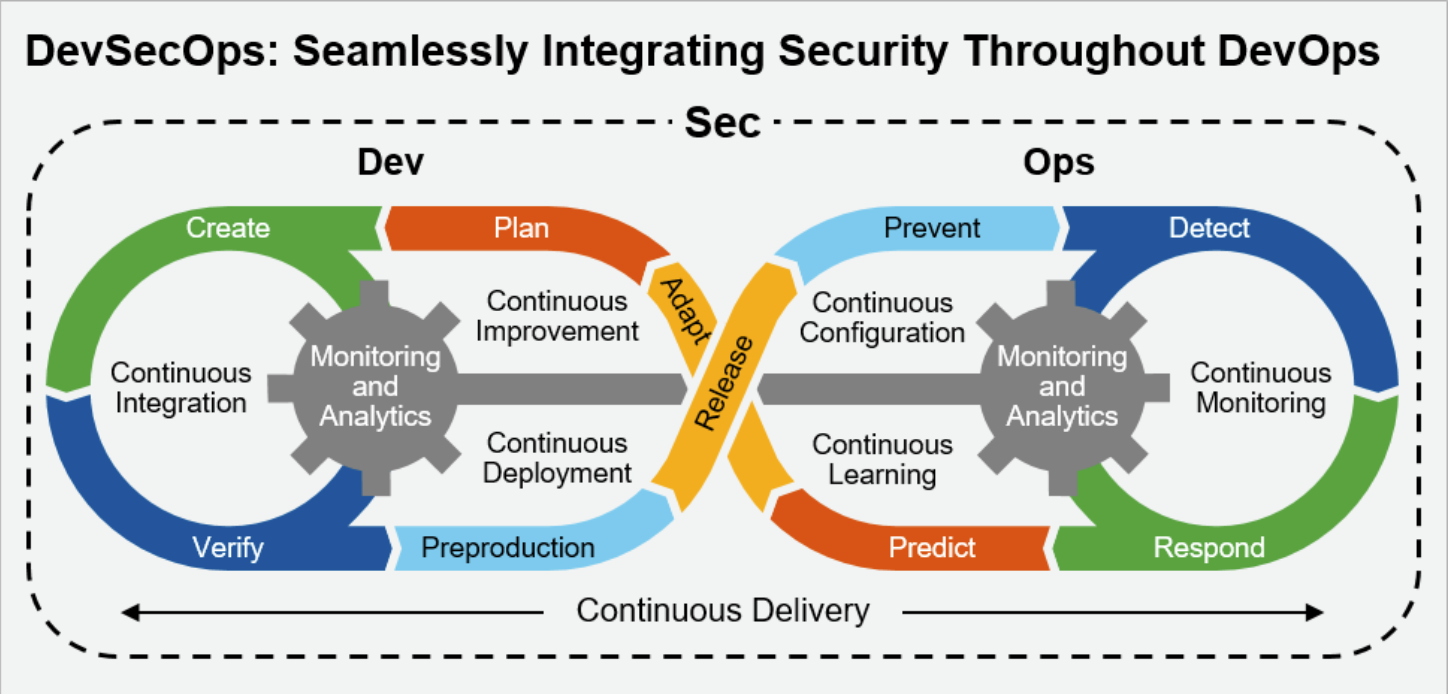
\includegraphics[width=\textwidth]{devsecops} 
  \caption{Ciclo de vida de desarrollo del software DevSecOps}
  \label{fig:DevSecOps-SDLC}
\end{figure}


%TODO: Revisar párrafo, un poco chapuza
Al igual que en el movimiento DevOps, esto se puede conseguir mediante la
incorporación de ``Jobs'' que revisen el estado del código generado durante el
desarrollo.  Aun así, la mejor forma de seguir esta filosofía es creando una
cultura que la reconozca y respalde, de forma que los desarrolladores no se
molestan al ver que el código tiene vulnerabilidades, sino que evolucionen,
mediante formaciones o reportes de los fallos de su código, a desarrollar de
forma segura.

Anteriormente, la seguridad formaba parte del último paso del ciclo de vida del
desarrollo de software, el mantenimiento.  Como consecuencia, en el momento en
el que se halla una vulnerabilidad de seguridad, o lo que es peor, un agente u
organización externos usan dicha vulnerabilidad para extraer información
sensible de los usuarios de la aplicación, los recursos necesarios para
arreglarla y el tiempo empleado en arreglarla, son muy elevados, al igual que el
estrés y la posible sanción relacionada con la intrusion en el sistema y la Ley
de Protección de Datos.  Este hecho es uno de los principales motivos por el que
las empresas que ya han adoptado el modelo DevOps, están apostando hacia el
modelo de desarrollo de software \gls{DevSecOps}.

Este cambio no es inmediato, se puede ver en la gráfica
inferior(\ref{fig:DevOps-DevSecOps-GTrends}), la comparativa
de búsquedas de Google con el termino \gls{DevOps} y \gls{DevSecOps}.

\begin{figure}[H]
  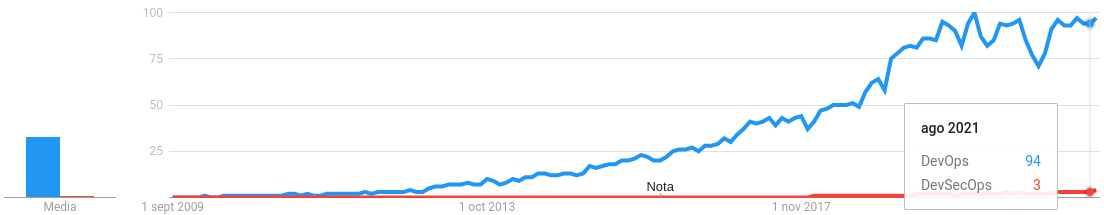
\includegraphics[width=\textwidth]{DevOps-DevSecOps-GTrends} 
  \caption{Comparativa Google Trends entre DevOps y DevSecOps}
  \label{fig:DevOps-DevSecOps-GTrends}
\end{figure}

Esta gráfica proporciona evidencias de que el movimiento hacia un ciclo de vida
seguro está empezando y muy posiblemente ofrezca una ventaja competitiva a
quienes lo adopten tempranamente frente a las demás empresas.

Como podemos observar en el diagrama anterior (\ref{fig:DevSecOps-SDLC}), el modelo
de desarrollo basado en una filosofía DevSecOps, mueve las comprobaciones de
seguridad desde la fase de mantenimiento, a la fase inicial, contemplando la
seguridad como uno más de los requisitos que se plantean en la fase de
planificación y conservando su importancia durante todo el ciclo de vida del
software.
En definitiva, la seguridad, pasa a ser una parte integral del ciclo
de vida de desarrollo del software. 

Para conseguir este propósito, los practicantes de dicha filosofía implementan
``jobs'', o tareas automatizadas relacionadas con la seguridad en el mismo
``Pipeline'', tan característico de DevOps.

Las ventajas que ofrece la metodología \gls{DevSecOps} son las siguientes:

\begin{itemize}
  \item{Reducción del tiempo medio en desplegar en producción}
  \item{Despliegues mas frecuentes}
  \item{Caracterización, monitorización y mitigación de riesgos durante todo el
    ciclo de vida del proyecto}
  \item{Actualización y arreglo de software a la velocidad de operación}
\end{itemize}

Las ventaja superiores son similares a las \gls{DevOps} ya que también reduce
el tiempo de despliegue y aumenta la frecuencia de despliegues, pero ademas de
proporcionar todas las ventajas de \gls{DevOps}, también proporciona las
ventajas de una seguridad integral a lo largo de toda la plataforma.
Esto aumenta la confianza el el producto y evita o informa de multitud de
vulnerabilidades en el entorno de producción, reduciendo así la exposición a
ataques de la aplicacion, con los beneficios que esto conlleva.

En los últimos años, el sector del software ha explotado con empresas como
GitHub, GitLab o GoCD, que proporcionan a los equipos de desarrollo las
herramientas básicas y los pilares fundamentales para que sus clientes adopten
una filosofía DevOps y DevSecOps en la construcción de
software.\cite{Google2019}. Un ejemplo de el uso de la filosofía DevSecOps es el
concepto llamado ``Abuser storie'' \cite{Bor2006} en el que se aplica la
seguridad en la fase de Planificación, a conceptos previos, como los ``User
Stories''. Un user story es una breve descripción escrita por el cliente de no
más de tres líneas sobre la funcionalidad que debe proporcionar la aplicacion.
\cite{XPUserStory} mientras que un ``abuser story'' es una extension de los
``User Stories'' contemplado por un ingeniero de seguridad para poder tomar
decisiones informadas en base al estado de la seguridad en el momento de su
definición. \cite{Bor2006}

Esta forma de replantearse la seguridad es exactamente el cambio de paradigma
necesario que lleva de la filosofía \gls{DevOps}, a la filosofía
\gls{DevSecOps}.


% Parte principal del documento
\chapter{Implementación del modelo DevSecOps}

En la primera sección de este capitulo, se pretende describir la forma en la que
se ha construido el pipeline DevSecOps, analizando cada una de las fases del
ciclo de desarrollo en su estado actual e identificando los problemas que
presenta.
Posteriormente, teniendo en cuenta los problemas descritos en la
sección anterior, se crea un pipeline conceptual, en el que se definen, a nivel
de seguridad las revisiones o \gls{job}s necesarios para que el \gls{pipeline}
conserve la practicalidad, pero asegure la seguridad y calidad del software.
Mas adelante se procede a analizar las tareas inferidas y asignarles un tiempo
de investigación y desarrollo estimado (L0) ademas de una prioridad de
desarrollo.
Una vez definidas las tareas, se ordenan y se crea la estrategia de
desarrollo necesaria, ademas de los objetivos a los que hay que llegar a medio y
largo plazo.
Para terminar, se definen una serie de indicadores, para medir los
resultados de los cambios que tenemos pensado implementar en el ciclo de vida
del desarrollo de software, a nivel de seguridad en Scalefast.

Los recursos compartidos en esta observación y subsecuente propuesta de ciclo de
vida seguro mediante \gls{DevSecOps} provienen de la experiencia acumulada en el
día a día de Scalefast.
De esta forma, la propuesta debe ser revisada por cualquier organización o
individuo que desee implementar un ciclo de vida similar.

En la segunda sección de este capitulo, se describe el desarrollo de una de
estas tareas (Concretamente, la implementación de un almacén de secretos con 
\href{https://www.hashicorp.com/products/vault}{HASHICORP Vault})
 desde su asignación, a su finalización, añadiéndola al
\gls{pipeline} para que pueda garantizar la seguridad y calidad del desarrollo
de nuestro producto, en Scalefast.

\section{Análisis del estado actual del pipeline} %DEFINICIÓN DEL PROBLEMA

En Scalefast, se sigue un modelo de desarrollo similar al descrito
anteriormente, en la metodología ágil.  Actualmente, la empresa tiene un
\textit{\gls{pipeline}} de integración continua, en el que se pasan varios
``jobs'' o pruebas automáticas en cada commit vinculado a un \acrfull{mr} que se
sube al repositorio de código.  
Un \textit{\gls{pipeline}} es la pieza clave del
ciclo de vida del software, responsable de asegurar la calidad de los
desarrollos que se integran a producción y que, de forma indirecta,
definen la calidad de la empresa.  De la misma forma, es importante recordar que el
desarrollo del \textit{\gls{pipeline}} debe seguir siempre el modelo de
desarrollo de software que él mismo promueve, es decir, el desarrollo iterativo e
incremental.  Dicho esto, es evidente que su desarrollo deberá seguir
siendo una prioridad de la empresa.  En vista de la progresión de Scalefast,
debemos evolucionar el pipeline, haciendo que tienda más hacia la integración y
despliegues continuos, centrándonos, además en el desarrollo de software en la
seguridad.  

Los esfuerzos por adoptar una filosofía \gls{DevOps} en Scalefast empiezan a
finales de 2019.
El progreso de Scalefast hacia la nueva metodología ha llevado a la compañía a
crear distintos ``Pipelines'' que revisan el estado del código, tanto cuando se
hace un \gls{merge} o \gls{MR}.
Ademas, tienen la capacidad de lanzar ``Pipelines'' de forma programática,
cuando se soliciten para revisar que las integraciones que se han hecho sobre
distintas ramas funcionan correctamente.

Los cambios estructurales en una organización conllevan una serie de factores no
cuantificables, como el tiempo que tarda una persona en asumir los nuevos
procesos y formas de desarrollo.
Por este motivo, Scalefast sigue en un estado temprano en la adopción de
una metodología \gls{DevSecOps}.
Se podría decir, por tanto que el tiempo necesario para que una organización
como Scalefast adopte la filosofía \gls{DevSecOps} en su integridad es mayor al
tiempo que se ha tenido hasta la fecha.

\subsection{Problemas encontrados y mejoras}

Una de las razones por las que se decide actualizar el \textit{\gls{pipeline}}
es porque se quiere promover el desarrollo seguro desde el inicio del ciclo de
vida del proyecto.  Actualmente, la forma que tenemos de revisar la seguridad
del proyecto es mediante un análisis manual de seguridad una vez ha
terminado el desarrollo del mismo.  

Por otro lado, los inconvenientes heredados de seguir
esta metodología de desarrollo se encuentran en el momento en el que aparece una
vulnerabilidad. Así pues, el plazo que se tarda en elaborar una solución
incluye: el tiempo en analizar el problema, la asignación del
desarrollador responsable, el planteamiento de la solución del problema, el
desarrollo de la misma, la revisión (para asegurar que el fallo esta
neutralizado) y la subsecuente revisión. La finalidad, pues, es asegurar que no
se han añadido fallos de regresión o nuevas vulnerabilidades.  En cambio, si se
incluye un analista de seguridad desde la fase de concepción del proyecto,
durante el ciclo de vida del desarrollo y se crean \textit{\gls{job}s}, para
analizar la parte mas automatizable del desarrollo, se reduce considerablemente
la probabilidad de encontrar un fallo en los últimos pasos del desarrollo del
proyecto.

Llegados a este punto, a medida que Scalefast ha crecido, se han identificado
una serie de problemas en el \textit{\gls{pipeline}} que usamos actualmente: 

\begin{itemize} 
  \item{Se pueden introducir cambios a producción manualmente} 
  \item{No se pueden repetir despliegues} 
  \item{No existe una forma estable de revertir los cambios añadidos a prod} 
  \item{No se revisa siempre el código de la misma forma} 
  \item{La revision es susceptible a modificaciones manuales} 
  \item{No se replican entornos entre fases (pruebas, \gls{staging} y producción)} 
  \item{No existe responsabilidad de código} 
  \item{No hay indicadores de calidad}
  \item{No ofrecemos visibilidad directa a distintos entornos}
  \item{No se ofrece una forma de despliegue de código continuo}
  \item{No existe una serie de herramientas automatizables destinadas a revisar
    la seguridad de la aplicación} 
\end{itemize}

Ademas de problemas encontrados en el \gls{pipeline}, también existen
inconvenientes relacionados con la arquitectura de la aplicacion, ya que esta es un
monolito.
La filosofía \gls{DevOps} funciona mejor con aplicaciones `Stateless'', ya que
estas se pueden escalar horizontalmente, no verticalmente, como la aplicacion
``Stateful'' que gestiona Scalefast.

Este documento se centra en los cambios que se deben hacer para llevar a
Scalefast hacia una metodología de trabajo \gls{DevSecOps}.
No obstante, en vista de los problemas mencionados anteriormente, Scalefast esta
llevando a cabo proyectos para migrar la aplicacion monolito a una aplicacion
``stateless'' basada en microservicios para poder obtener los beneficios
esperados de esta nueva metodología.
De entre estos problemas detectados, algunos se pueden solventar añadiendo
herramientas directamente y otros son problemas culturales, que se tienen que
abordar de distinta forma.


\section{Desarrollo conceptual del pipeline de seguridad}

Para llevar a cabo una transformación metodológica como la que se plantea, 
en la que se va a ver afectada gran parte de la organización en la forma en la
que se desarrolla el software, deben existir cuatro pilares fundamentales sobre 
los que se va a tener que sostener.
Estos se reflejan en el diagrama inferior.

\begin{figure}[H] 
  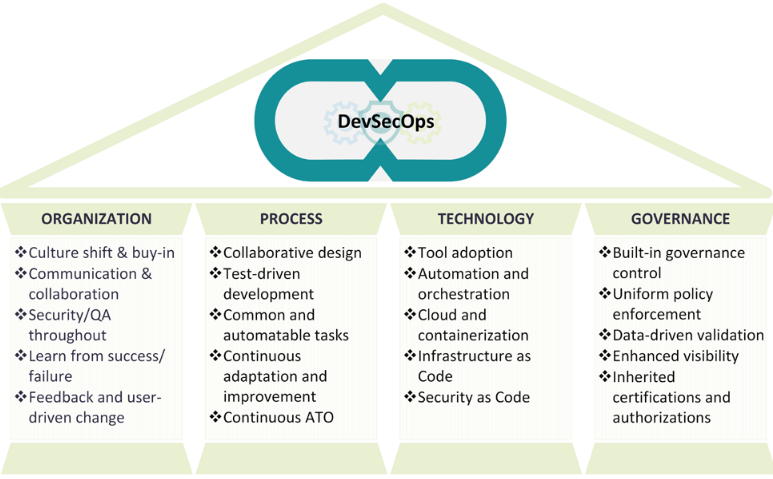
\includegraphics[width=\textwidth]{DevSecOps-pillars}
  \caption{Pilares sobre los que se sustenta DevSecOps}
  \label{fig:DevSecOps-pillars}
\end{figure}

%TODO: Seguir escribiendo por aquí las cosas que deben pasar para que se
%implante correctamente una organización DevSecOps.
A nivel \textbf{organizativo}, en Scalefast se ha creado un presupuesto para el equipo
DevOps, ademas, los directivos de la empresa apoyan la dirección que esta
tomando el equipo.
Aunque haya ciertas características que se cumplan, también existen otras que
no, como por ejemplo los indicadores de rendimiento.
Estos indicadores son necesarios para poder medir el impacto que se hace desde
el equipo y tener datos reales del cambio que es capaz de hacer una metodología
\gls{DevSecOps}.

En cuanto a \textbf{proceso}, la organización cumple gran parte de los
requisitos o indicadores de una buena base.

La \textbf{tecnología} que se usa en Scalefast sigue una evolución prometedora,
se automatiza la mayor parte de las tareas del Pipeline y los nuevos
desarrollos, se implementan, en la medida de lo posible teniendo en cuenta la
seguridad.

Durante el ciclo de vida de Software, se asumen ciertos riesgos.
La gestión y observación de los mismos se llama \textbf{gobernanza}.
Actualmente, en Scalefast, no existe un sistema de gobernanza de datos maduro a
lo largo de todo el proceso de desarrollo de Software.

Como podemos ver, para adoptar una metodología \gls{DevSecOps} y poder conseguir
todos los beneficios que esta nos promete, hacen falta alinear prácticamente a 
toda la parte técnica de la organization.

%TODO: Revisar, a ver que pasa

\subsection{Tareas DevSecOps para el Pipeline}

Recientemente, Mike Ensor y Drew Stevens publicaron un ``paper'' titulado
``Shifting left on security''.  En él, explican las diferentes fases de el ciclo
de vida del software, y como añadir elementos de seguridad a lo largo del
``pipeline''.  Desde la planificación del proyecto hasta el despliegue del
mismo.  Algunas de las técnicas que recomiendan en su ``paper'' tienen gran
importancia. Por ejemplo,  el uso de registros de imágenes privadas, cuyas
imágenes y recursos están identificadas y verificadas a la hora de desplegarse;
el análisis estático y dinámico del código que se escribe de forma automatizada;
el despliegue del mismo binario que solamente pueda ser desplegado si es firmado
de forma criptográfica por el responsable de despliegues. (\cite{Ensor2021})

En esta sección, se describen más en detalle dichas herramientas y se documenta
el proceso de creación del pipeline a nivel conceptual.

Existen una gran variedad de tareas o comprobaciones disponibles para mejorar el
ciclo de vida del Software a nivel de seguridad.  Por cada tarea, existen
multitud de herramientas que la pueden realizar a mayor o menor medida, este es
el motivo por el cual nos centramos en las tareas a nivel conceptual ya que cada
equipo va a disponer de un presupuesto o tiempo determinados.  Nuestro propósito
final debe ser siempre la automatización de dichas herramientas para incluirlas
en la fase adecuada del Pipeline de forma que a medida que el código que se
registra en el sistema de control de versiones va pasando cada una de las fases
del Pipeline, vamos aumentando nuestro nivel de confianza en el mismo.

Los distintos tipos de revisiones de seguridad que se pueden realizar sobre el
código provienen de las distintas formas que se han conseguido vulnerar los
sistemas en el pasado o de ataques conceptuales que podrían realizarse sobre la
plataforma.  En el sector de la seguridad, el atacante siempre tiene la ventaja,
puesto a que nunca se puede tener un sistema completamente seguro debido a la
cantidad de dependencias, fallos de seguridad a la hora del desarrollo y
sistemas sobre los que esta construido el proyecto.  Dicho esto, se pueden tomar
medidas preventivas, para que nuestros sistemas no queden expuestos a ataques
conocidos.  Con esta finalidad en mente, se automatizan las tareas a modo de
Pipeline para prevenir errores detectables con análisis automáticos.

% Tipos de revisiones que se pueden hacer. (Que analiza que herramienta)
Siguiendo la investigación, se han seleccionado varias formas de revision del
Pipeline que pueden ser de gran utilidad para asegurar la calidad a nivel de
seguridad del código.  Estas se pueden dividir a grandes rasgos en
Infraestructura y aplicacion.

Como explican Emerson y Stevens, para poder garantizar la protección y
seguridad del software sobre el que se esta ejecutando el código de la
organización es necesario disponer con de una infraestructura segura.  Hoy en
día, esta tarea pasa a ser responsabilidad de proveedores de infraestructura en
la nube, como pueden ser \href{https://aws.amazon.com/}{AWS} o
\href{https://console.cloud.google.com/}{GCP}.  No obstante, si que hay una
serie de comprobaciones que podemos realizar sobre contenedores.  Posteriormente
se entra en detalle sobre este aspecto.

Por otro lado, como no es necesario revisar la arquitectura sobre la que corre
la aplicación cada vez que se ejecuta un \Gls{pipeline} no se va a entrar en
detalle sobre las formas que existen para protegerla.

Podemos entonces reducir en campo de revisiones a la capa de aplicacion.  En
esta capa, según la fase de desarrollo en la que nos encontremos, debemos
prestar atención a distintas areas.

% Hacer ver la necesidad de usar herramientas de seguridad automatizadas, e
% implementarlas en el ciclo de vida del software.
Según revela el estudio anual \nocite{sonatype2020} realizado en 2020 por
\href{https://sonatype.com}{Sonatype}, podemos observar que la mayor parte de
las empresas están concienciadas con la seguridad, pero que solo son las que
tienen una actitud mas madura respecto a DevOps, las que adoptan una serie de
tecnologías mas actualizadas como pueden ser análisis de contenedores o
análisis dinámico.

\begin{figure}[H] 
  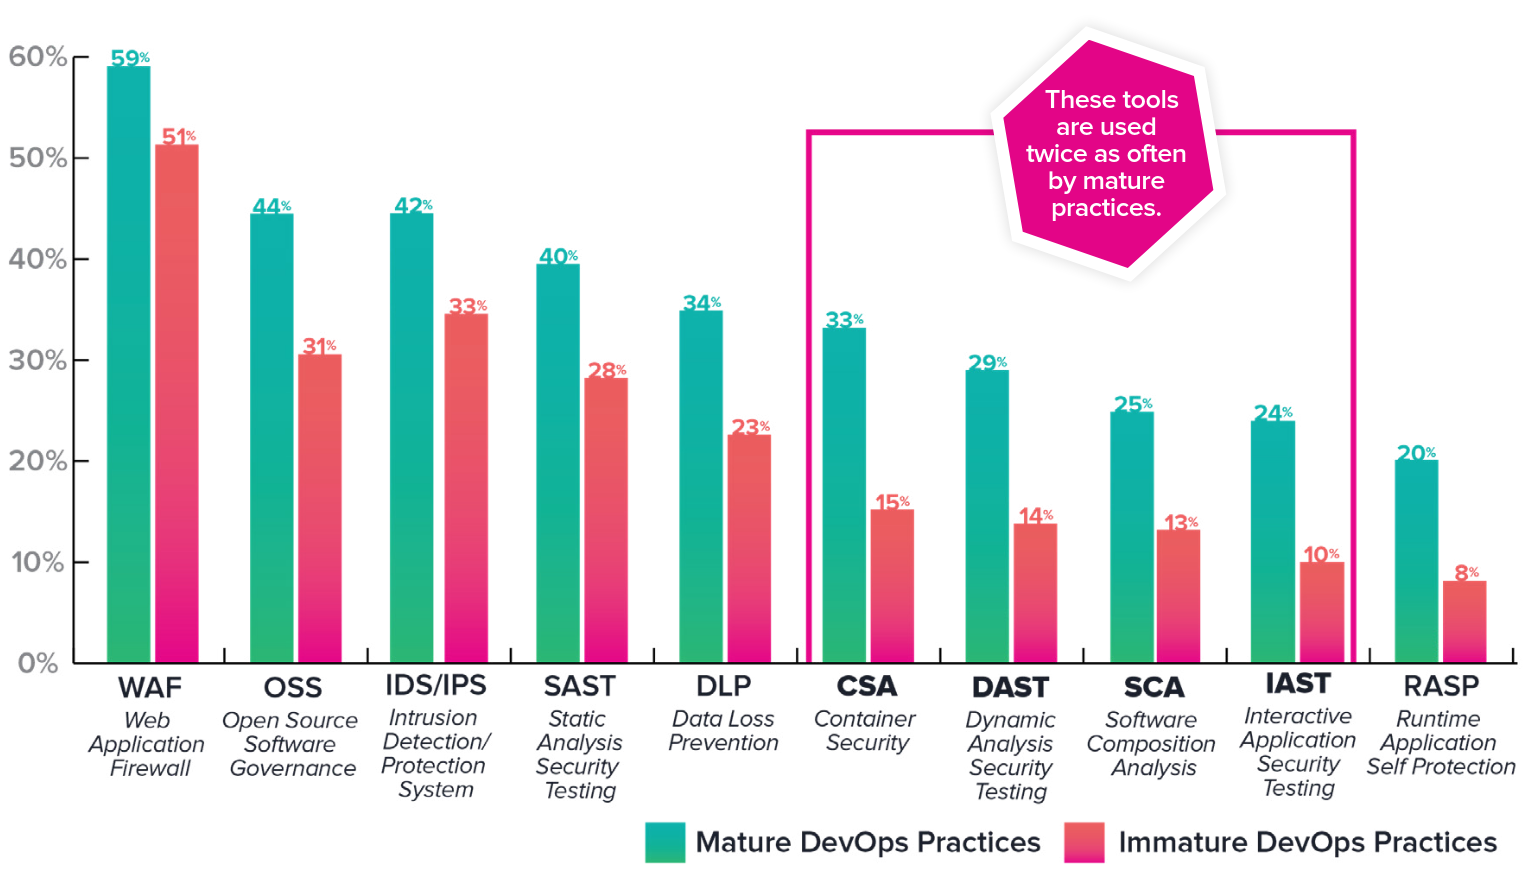
\includegraphics[width=\textwidth]{sonatype-tools}
  \caption{Adopción de herramientas de seguridad por las empresas}
  \label{fig:sonatype-tools}
\end{figure}

En la gráfica superior (\ref{fig:sonatype-tools}) se resalta que las empresas
maduras en el campo DevOps usan tecnologías automatizadas como \gls{CSA},
\gls{DAST}, \gls{SCA} y \gls{IAST}.  
Estos datos validan los mostrados en la gráfica
(\ref{fig:DevOps-DevSecOps-GTrends}), aunque la metodología \gls{DevOps} si que
esta mas extendida, la metodología \gls{DevSecOps} sigue siendo novedosa y son
solo las empresas mas maduras o evolucionadas, las que adoptan estas practicas.

Dado que se pretende rediseñar el \gls{SDLC} para que tenga en
cuenta la seguridad a la hora de desarrollar nuestra plataforma, es interesante
revisar estas aplicaciones, para ver si se ajustan a los requisitos de calidad
que pretende obtener Scalefast con este cambio de ciclo de desarrollo.
A continuación se analizan, entre otras, estas tecnologías.

\subsubsection{Definición y análisis del proyecto} \label{definicionyanalisis}

En esta fase, mucha mas organizativa del ciclo de vida del desarrollo, no se
pueden crear tareas automatizables para revisar la seguridad del software, ya
que este aun no ha sido escrito.  En su contra, las técnicas que debemos aplicar
son de carácter manual.

Entre las técnicas que se pueden aplicar, existe el modelado de riesgos, y las
historias de abuso.  Esta primera técnica consiste en seguir un modelo, como por
ejemplo \gls{STRIDE}, que sirve para analizar y encontrar los riesgos de
seguridad en un sistema.  El modelo \gls{STRIDE} garantiza que si se separa el
producto en sus componentes y cada uno de estos cumple con los seis requisitos
de \gls{STRIDE} \cite{Loren1999}, (Spoofing, Tampering, Repudiation, Information
Disclosure, Denial of Service y Elevation of privilege), entonces, el producto
es seguro.

En el segundo caso, las historias de abuso, son casos particulares de historias
de usuario.  En 2005, Johan Peeters introduce este concepto, definiéndolo de la
siguiente manera: Las historias de abuso identifican la forma en la que los
atacantes pueden abusar del sistema y comprometer los recursos de los
accionistas.  Por tanto, especifican requisitos de seguridad del sistema.  Al
igual que las historias de usuario, lo hacen breve e informalmente.
\cite{Peeters2005}

\subsubsection{Desarrollo del código fuente}
 
%TODO: Análisis de secretos
Cuando se desarrolla código, existen una serie de consideraciones que debemos
tener en cuenta.  Debido a la naturaleza perezosa de las personas, se tienden a
dejar contraseñas, configuraciones o claves de \gls{API} en los propios archivos
de texto sobre los que se escribe el código.  Estos archivos de texto, se suben
a un sistema de control de versiones.  Este flujo almacena una nueva version del
archivo cada vez que se guarda en el sistema de control de versiones, por lo
tanto, esta información sensible permanecerá indefinidamente en el historial de
cambios del sistema.  Para prevenir esto, se han creado herramientas que
previenen que el desarrollador guarde en el sistema de control de versiones
dicha información sensible.  Estas herramientas se llaman analizadores de
secretos.

% Tests funcionales
En esta sección, se pretende poder revisar el código fuente mientras este sigue
en desarrollo, por tanto, las pruebas darán un resultado negativo hasta que se
hayan completado todos los requisitos funcionales representados en los pipelines
como tests de funcionalidad.

% Composición del código
Ademas de la funcionalidad, se puede revisar la composición del software.  Se
analizan las librerías y dependencias externas que utiliza el software que
estamos construyendo en nuestro proyecto en búsqueda de vulnerabilidades y
posibles vectores de ataque introducidos por las dependencias o librerías.  Este
tipo de técnica se llama análisis de composición de software, o \gls{SCA}.  La
finalidad es asegurar que los componentes de nuestro sistema no tienen
vulnerabilidades conocidas, o que si las tienen, estemos preparados para asumir
el riesgo que introducen en nuestro sistema.  A medida que han ido evolucionando
las herramientas que se encargan de realizar los análisis de composición de
software, también han ido evolucionando la cantidad de opciones que incluyen.
Hoy en día, estas herramientas son capaces de detectar que nuestro sistema usa
una librería que incluye una vulnerabilidad y actualizar dicha librería para que
nuestro sistema ya no presente esta vulnerabilidad, automatizando todo el
proceso de análisis de vulnerabilidades de los componentes de nuestro sistema y
posterior actualización de los mismos.

%TODO: Análisis de código estático
Otra herramienta que puede ayudar en el análisis de vulnerabilidades en el
sistema, es el análisis de código estático, o \gls{SAST}.  Aunque algunas
características de esta herramienta se solapan con las características de otras
herramientas automatizadas de análisis de código, siempre se debería usar.  Es
considerada la herramienta de análisis de código por defecto en los ciclos de
vida del software, y asienta las bases de estos.

%TODO: Peer review
Finalmente, se incorpora al ciclo de vida del software una tarea de revision del
código escrito por un compañero, para validar que el código esta bien escrito y
este no presenta ningún problema propio de la plataforma no detectable por las
herramientas de análisis automáticas. Todas estas herramientas, de las que se ha
hablado hasta ahora, se solapan en alguna funcionalidad unas con otras, pero las
ventajas de crear un ciclo de vida seguro aunando cada una de estas
herramientas, sobrepasa las 


\subsubsection{Testeo del código} \label{testeodecodigo}

Para llegar a esta fase del \gls{SDLC}, el código ha debido pasar
satisfactoriamente por la fase de definición y análisis y por la fase de
desarrollo.  En cada una de estas dos fases, se revisa, de forma manual o
automatizada varias secciones de la aplicación.  Esto indica que la confianza en
el código incrementa.  En el momento en el que pase esta fase, la probabilidad
con la que el código en question se despliegue al entorno de producción se eleva
considerablemente.  Es por esto, que esta fase debe ser mas complicada de
superar que las dos fases anteriores.  En esta fase entran en juego tecnologías
de análisis como \gls{SAST}, \gls{CSA}, \gls{DAST}, tests no funcionales y tests
específicos de la plataforma de Scalefast.

%SAST
El análisis de código estático del proyecto entero difiere del análisis estático
de la fase anterior ya que este tiene en consideración el proyecto entero, no
solamente la parte en la que está trabajando el desarrollador o grupo de
desarrolladores.  Ademas de asegurar una buena practica de programación, esta
revision permite mantener una medida de calidad general del proyecto, comparable
a lo largo del tiempo y versiones.  En el momento en el que todo el proyecto no
supere un valor establecido con anterioridad, este commit no pasará el
\gls{pipeline} y los desarrolladores deberán arreglar el problema.  El commit
tampoco pasará la prueba de código estático si no sigue un estilo previamente
definido o si la herramienta de análisis detecta posibles indicadores de
programación insegura.

%CSA TODO: Acabar de escribir por aquí
En 2019, ya existían indicios de que la industria iba a girar en torno a los
contenedores.
Así lo indican los datos obtenidos por el estudio realizado por Sandy Carielli
para Forrester:
``as of 2019, 33\% of global developers indicated that their development
organizations currently use containers, and another 25\% said they want to do so
over the next 12 months.''(\cite{Carielli2020}).
El problema con esta gran adopción y crecida en popularidad es que la seguridad
queda relegada a un segundo plano.
Las empresas de seguridad no pueden desarrollar productos lo suficientemente
rápido como para suplir la trayectoria hacia la nueva tecnología, en este caso,
los contenedores y la industria acaba adaptando medidas de seguridad antiguas a
estas nuevas tecnologías.
Una de las nuevas medidas de seguridad creada específicamente para contenedores,
es el análisis de contenedores.
También llamado \gls{CSA}.
Estas herramientas automatizables analizan las capas de las que están formados los
contenedores en búsqueda de vulnerabilidades.
Si las encuentran, notifican a los propietarios de los mismos.
En el \gls{SDLC} que se pretende implementar en Scalefast, estas herramientas
forman parte del \gls{pipeline}.
Incluyendo este tipo de análisis en los \gls{pipeline}s, pretendemos asentar una
base segura, sobre la que luego se despliega la aplicación. 
Una de las posibles herramientas de análisis de contenedores es Snyk, que, en
colaboración con Docker, permite analizar las imágenes con un solo comando.
Otra, de código libre, es \href{https://github.com/docker/docker-bench-security}{docker-bench-security.}

%DAST
La mayor parte de ataques que debe poder soportar la aplicación son ataques que
se ejecutaran mientras esta está en ejecución.
Además de un análisis estático de código, también se debe analizar la aplicación
de forma dinámica.
Este tipo de análisis se llama Tests de seguridad de aplicación
dinámicos o \gls{DAST}.
Este análisis revisa que la aplicación sea resistente a ataques interactivos,
como \gls{XSS} o \gls{SQLi}.
Estas herramientas analizan las respuestas que proporciona la aplicación y
según el tipo de respuesta, la aplicación de análisis dinámico comprueba si la
aplicación es o no vulnerable al ataque que se le intenta aplicar.
Al añadir esta herramienta al \gls{pipeline}, en caso de que el ataque se
realice con éxito, el \gls{pipeline} falla y el equipo encargado de ese
desarrollo deberá solucionar el fallo.

%Non-funcional tests
En cualquier aplicación que se cree, se deben especificar tanto los requisitos
funcionales como los no funcionales ya que de nada sirve tener una aplicación
bancaria que cumple todos los requisitos funcionales, pero no consigue
mantenerse estable cuando se conectan más de tres personas en el mismo momento.
Los requisitos no funcionales definen justamente estas características.
Algunos de los requisitos no funcionales se pueden interpretar como
\acrfull{SLO}, o objetivos que debe cumplir la aplicación.
Revisando estas característica durante el ciclo de desarrollo, y no al final, se
deben poder detectar con anterioridad estos problemas, en caso de que surjan.
Existen varios tipos de tests no funcionales, cada uno revisa una parte de la
aplicación.
Los \textbf{tests de rendimiento} revisan que la aplicación responde a las peticiones en
un tiempo inferior o igual a lo estipulado.
Los \textbf{tests de carga} revisan que la aplicación funciona correctamente y responde en
un tiempo inferior o igual que el estipulado a las peticiones que le entran
mientras está siendo usada por el máximo numero de usuarios posible en ese mismo
instante. Bajo este tipo de estrés, la aplicacion no debería aumentar el tiempo
de respuesta.
Otro tipo de test no funcional es el \textbf{test de estrés}.
Este tipo de tests miden la respuesta de la aplicacion a un nivel de trafico que
excede lo esperado. Sirve para medir la capacidad de respuesta de la aplicacion
en situaciones criticas.
Es necesario tener en cuenta que cada proyecto debe tener sus propios requisitos no
funcionales, por tanto, estas herramientas se deben configurar de acorde a las
característica deseadas, pactadas tanto por el cliente como por la organización
en la fase de definición y análisis del proyecto (\ref{definicionyanalisis}).


%Platform-specific tests (Common errors with our programming style, and
%plataforma)
Además de los tests mencionados anteriormente, en Scalefast se ha decidido crear
una serie de pruebas o revisiones que controlen aspectos específicos de nuestra
plataforma.
Esto incluye la revision de fallos comunes realizados por los desarrolladores,
archivos de configuración que no deberían estar subidos al control de versiones
o parámetros de configuración puestos para revisar el código en la fase de
desarrollo, no la de producción.
Todas estas revisiones se pueden automatizar en un script y poner como una tarea
mas en la fase de testeo del \gls{pipeline}. 

Una vez el desarrollo destinado al entorno de producción han pasado por
todas estas fases (Definición y análisis del proyecto, Desarrollo del código
fuente y testeo del código) del ciclo de vida del software y sus respectivas
revisiones automáticas en forma de tareas dentro del \gls{pipeline} de
desarrollo, la confianza en el código ya es muy alta.

\subsubsection{Despliegue} 

Al ser un \gls{pipeline} centrado en la seguridad de la aplicación, una de las tareas
que se pueden realizar en esta fase consiste en una prueba de penetración,
también llamada \gls{PenTest} hacia la aplicación.
Esta prueba consiste en analizar las vulnerabilidades reportadas por las
herramientas de análisis estático o dinámico, ademas de un análisis manual
exhaustivo en busca de cualquier vulnerabilidad que pueda llegar a
materializarse en una intrusion, con las consecuencias que esto conlleva.  
Dependiendo de la importancia de la misma, las característica que tiene y el
cliente al que va a ser destinado (Ya que puede ser una aplicacion interna o
externa) se puede realizar una prueba de penetración sobre la aplicacion.

Ademas de la prueba de penetración, si el proyecto esta desarrollado con
contenedores, entonces se deberá realizar una prueba de seguridad de
contenedores o \gls{CSA}.
Aunque esta prueba ya se ha descrito en la fase de testeo de código,
(\ref{testeodecodigo}) es importante realizarla en cada una de las fases en las
que se crea o usa un contenedor distinto.
Esto se debe a que, siguiendo las buena practicas, ``as images head
to production you should remove everything that in’t absolutely necessary''
(\cite{Armstrong2020}).
La razón por la que se sugiere reducir las capas en las imágenes que van a
ejecutar el código en el entorno de producción es para eliminar vulnerabilidades
introducidas por frameworks o aplicaciones que no son necesarias para que se
ejecute el código en producción.
Al reducir el numero de vulnerabilidades en los contenedores que ejecutan el
código en producción, será más complicado que los atacantes encuentren o usen
una vulnerabilidad para ganar acceso a nuestro sistema.

Una vez el código ha superado todas las tareas que contiene el \gls{pipeline}
del \gls{SDLC}, ya se puede desplegar en producción.
Todo el esfuerzo que se ha hecho en anterioridad es para que en este momento, el
despliegue y mantenimiento de esta aplicación o cambio sea lo más sencillo
posible.

No obstante, todas las precauciones son pocas y pueden ocurrir casos en los que
el proyecto desplegado haya pasado todas las pruebas, pero haya causado
problemas en el entorno de producción.

Herramientas como \href{https://sensu.io/}{sensu} sirven para monitorizar el
despliegue y verificar que el cambio no ha desestabilizado el entorno de
producción.

\subsubsection{Monitorización} \label{monitorizacion}

Adema de supervisar la plataforma instantes antes, durante y después de un
despliegue, esta se debe monitorizar constantemente.

Gran parte de las tareas que ocurren en esta fase deben de ser continuas.
En esta fase, se debe revisar el estado general de la aplicación -- asegurando
su estabilidad -- aunque haya variaciones no funcionales que pongan a prueba la
aplicación, como el nivel de trafico que debe gestionar en un momento dado.
De estas tareas, normalmente se encarga el \acrfull{SRE}.

Para llevar esta tarea a cabo, se emplean herramientas de análisis de recursos,
como analizadores de disponibilidad.
Estas herramientas lanzan consultas predefinidas a la aplicación y miden el
tiempo de respuesta.
Este tiempo se contrasta con tiempos de respuesta pasados y se dibuja una
gráfica con estos datos.
Algunas herramientas mas avanzadas de monitorización, notifican a los analistas
en el momento en el que los tiempos de respuesta se desvían de los esperados.

Al igual que se mide la disponibilidad constantemente, también se debe medir las
vulnerabilidades a las que esta expuesta nuestra aplicación.
Aunque no se haya actualizado la aplicación, se pueden encontrar fallos de
seguridad en módulos que componen la aplicación, por tanto, es interesante
mantener una lista actualizada de las vulnerabilidades que contiene la
aplicación en todo momento.

%Conclusion
Habiendo analizado todos los tipos de revisiones y aplicaciones que se pueden
usar en el ciclo de vida del software, podemos concluir que todas estas
aplicaciones automatizadas centradas en la seguridad promueven un desarrollo
mucho mas consciente, intencionado y seguro.  Usando este tipo de políticas, se
promueven las buenas practicas de programación y el seguimiento de los
estándares de Scalefast.

\subsection{Creación conceptual del pipeline}

%TODO: Darle mucha mas luz a esta seccion 

Habiendo terminado la investigación inicial que resume las aplicaciones o tareas
usadas en la industria en el ciclo de vida del software, se procede a documentar
el ciclo de vida del software que se quiere implementar en Scalefast.
Esta documentación, una vez terminada se re-interpreta en forma de diagrama.
La intención del diagrama destinado a los miembros del equipo de
\acrfull{AppSec}, es resumir de un vistazo la meta a la que debemos llegar.
Por tanto, este diagrama debe representar todo el ciclo de vida del desarrollo,
desde la fase de definición y análisis del proyecto hasta la fase de
monitorización del mismo.
 
Durante la redacción del documento de ciclo de vida del software a nivel de
seguridad, se sigue la filosofía de llevar la seguridad a la izquierda porque
``By better integrating information security (InfoSec) objectives into daily
work, teams can achieve higher levels of software delivery performance and build
more secure systems'' (\cite{GoogleDOT})
por lo contrario, si encontrásemos ese error en una fase más avanzada del
desarrollo, este mismo cambio requeriría mas esfuerzo, mas tiempo y mas dinero
para solucionarse.

Por ejemplo, si encontramos duplicidad de código cuando este está desplegado en
producción, se tiene que crear un desarrollo nuevo, con todas sus fases
(Definición, Commit, Testeo, Despliegue y Monitorización), mientras que si
encontramos la misma duplicidad de código en la fase de desarrollo, el
desarrollador puede cambiar en ese momento el código que esta duplicado y este
nunca llegara a producción reduciendo así el tiempo destinado a esa misma tarea
además de las posibles repercusiones de seguridad que puedan suponer para
producción. 

A continuación se presenta el diagrama que resume el documento del \gls{SDLC},
más adelante se procede a explicar sus fases y composición.

\begin{figure}[H] 
  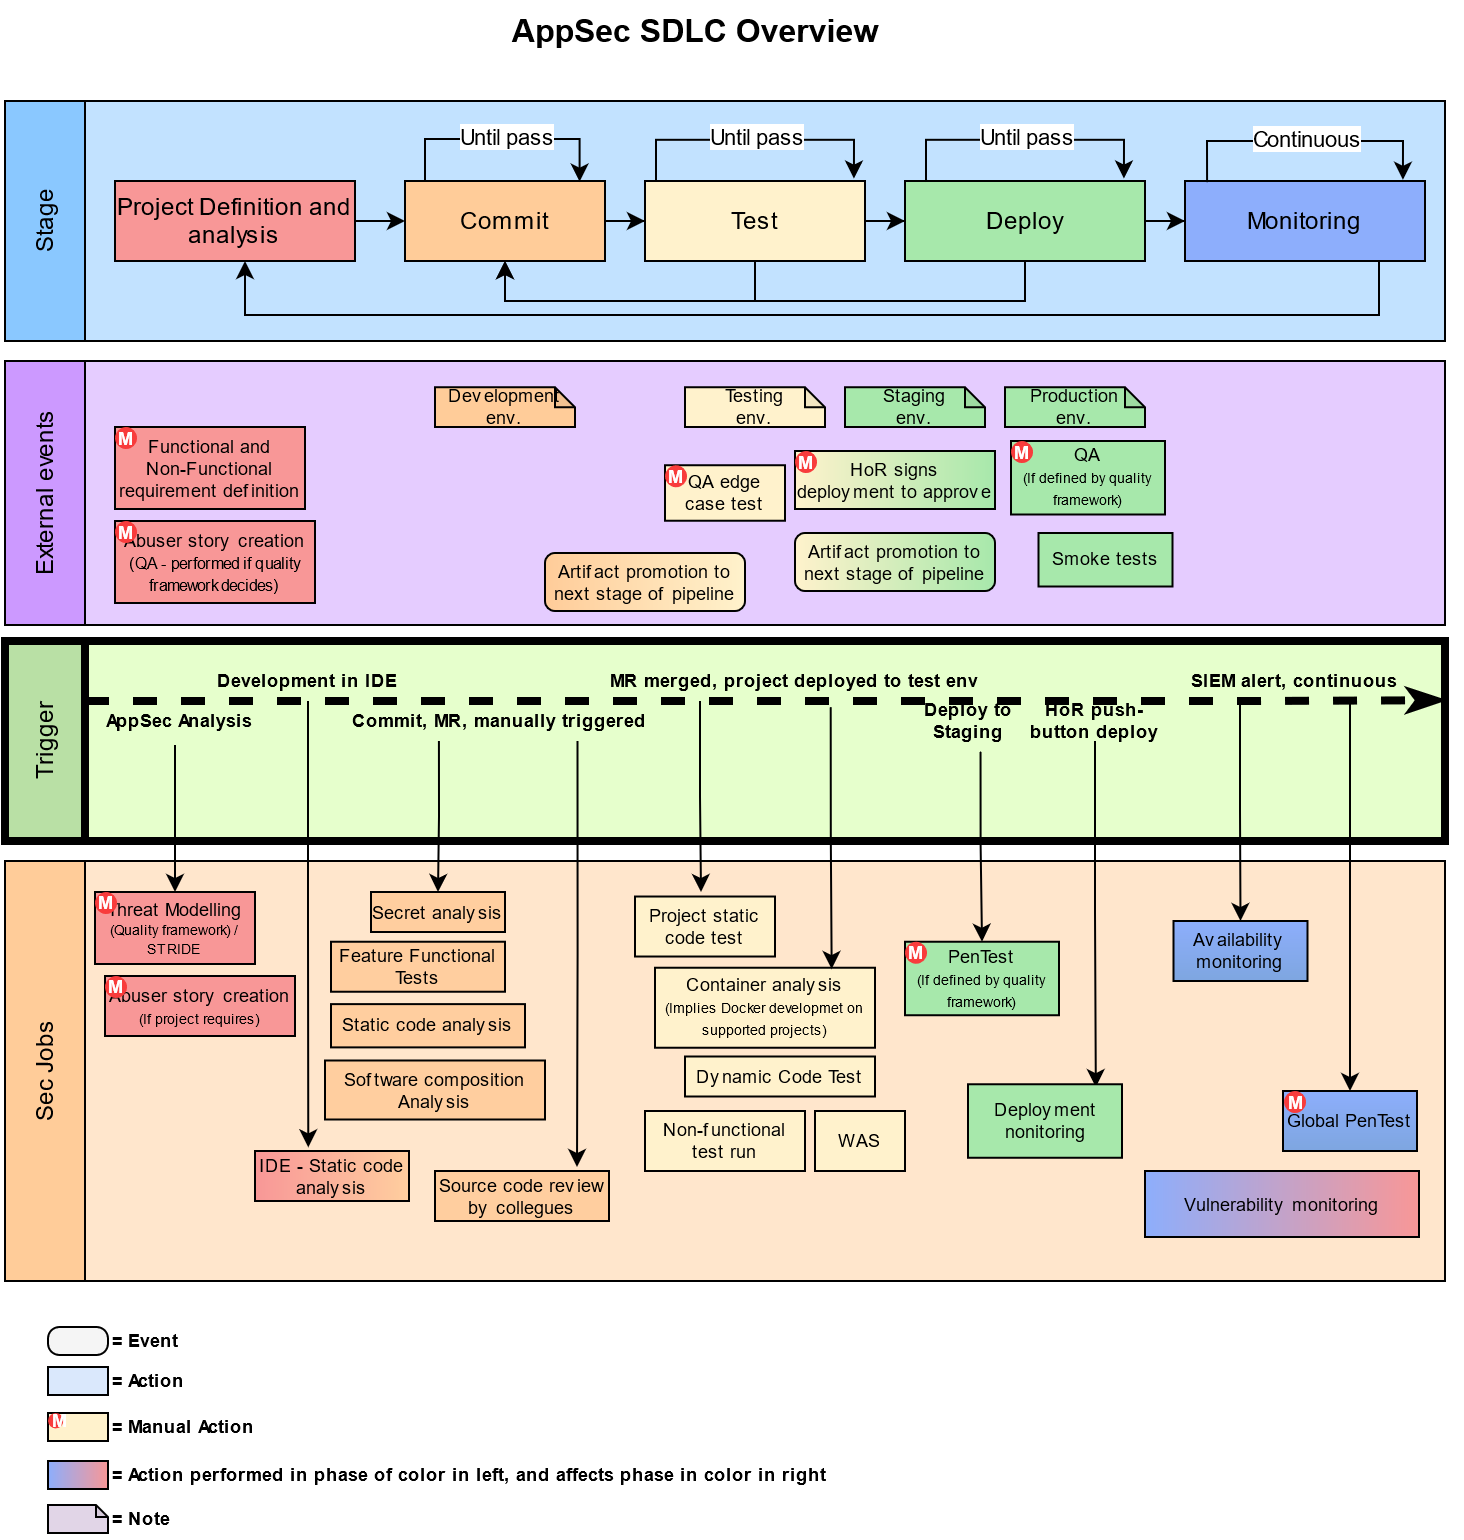
\includegraphics[width=\textwidth]{SDLC-Sec}
  \label{fig:SDLCOverview}
\end{figure}

Como podemos ver en el diagrama, este está dividido en varias filas.  Cada una
de estas filas agrupa una serie de \textbf{fases, eventos, detonantes}, o
\textbf{tareas} que ocurren a medida que se desenvuelve el ciclo de vida del
proyecto.

En las siguientes secciones, se describen las partes del diagrama, para
lograr una comprensión global del mismo.  Recordemos que la finalidad de este
diagrama es proporcionar una vision idílica del estado al que queremos llegar.
De este diagrama, se van a extrapolar las tareas necesarias y se les va a
asignar una prioridad y un tiempo de desarrollo. 

\subsubsection{Fase} 

En esta parte del diagrama, se representa la parte mas abstracta, o de alto
nivel del ciclo de vida del desarrollo.  Se introducen los estados.  La
definición del proyecto, la fase de desarrollo, la fase de pruebas, la fase de
despliegue y la fase de mantenimiento.  En esta metodología, todos los
desarrollos son iterativos e incrementales.  Esta característica intrínseca del
desarrollo ágil tiende a crear un desarrollo cíclico.  De ahí, las flechas ínter
conexas entre las fases.

Entrando mas en detalle, en la sección de definición y análisis del desarrollo,
se reúnen los responsables de cada área que se va a ocupar del desarrollo con el
cliente y se especifican las características del proyecto, requisitos
funcionales y no funcionales, además del tiempo de desarrollo estimado.  Cada
proyecto esta compuesto de funcionalidades y cada una de estas funcionalidades,
a su vez, están divididas en tareas.  Una vez está el proyecto completamente
definido se divide en funcionalidades y se les asigna a los equipos estas
funcionalidades.  Cada miembro de un equipo se puede encargar de una o varias
tareas.  Cuando una o todas las tareas han sido completadas, se pasa a la fase
de pruebas.  Es importante remarcar que cada tarea pasa a su vez por cada una de
las secciones de desarrollo.  A nivel de desarrollo de una tarea individual, el
desarrollador implementa pruebas unitarias, para asegurar que cumple los
requisitos especificados y cuando acaba el desarrollo, despliega sus cambios a
una maquina de integración, en la que se pasara otra fase de tests, esta vez más
general, asegurando que se cumplen las funcionalidades.  En el momento en el que
todas las funcionalidades han sido implementadas, se proceda a la fase de
despliegue.  En esta fase, se pone en el entorno de producción la funcionalidad
implementada.  Seguida de esta fase, se monitorizan los cambios añadidos, para
asegurara que no se han producido fallos de regresión y que todo funciona como
debe.  En el caso extremo en el que los cambios dejen inoperative el entorno de
producción, se quitan los cambios de producción para estabilizarlo y se crean
nuevas tareas para solucionar los fallos.  En el caso en el que se detecten
nuevos fallos no críticos, se crean nuevas tareas, también llamadas bugs, que se
deben arreglar, y estas vuelven a pasar por todo el ciclo de desarrollo.

En cada una de estas secciones, se ha establecido una serie de revisiones o
tareas para asegurar que la calidad de la seguridad es la mejor posible.  En
combinación con estas tareas, también se debe tener en cuenta las tareas que no
tienen relación con la seguridad, no añadidas a este gráfico, por motivos de
complejidad y acotación.

\subsubsection{Eventos}

Una vez vista la sección mas teórica, se presentan los eventos externos.  Estos
no necesariamente tienen una conexión directa con la seguridad.  Su principal
función es contextualizar el diagrama.  En esta sección, se introduce el
concepto de entornos.  Estos entornos, representados por un rectángulo con el
borde superior derecho doblado simbolizan la arquitectura sobre la que se debe
ejecutar el desarrollo.  En cada sección del ciclo de vida de desarrollo, se
debe usar un entorno distinto. Este estrategia de desarrollo se centra en 

Minimizar la exposición a vulnerabilidades adquiridas por las dependencias que
componen las imágenes o contenedores que usa la aplicación.
Además, al ejecutar la aplicación en cada uno de los entornos repetidamente --
una por cada \gls{commit} -- y la necesidad de que el \gls{commit} supere todas
las tareas del \gls{pipeline}, implica que el entorno sobre el que se ejecuta la
aplicación se ha desplegado múltiples veces.  Esto proporciona un nivel de
confianza explícitamente acumulada que nos sugiere que los despliegues no van a
romper la aplicación en el entorno de producción porque ya se ha despegado dicha
aplicación en el mismo entorno de un \gls{pipeline} anterior.  Como beneficio a
nivel de seguridad, desplegar el proyecto en un entorno de staging, proporciona
al analista de seguridad la opción de realizar cualquier tipo de comprobación
necesaria.  De este modo, se pueden realizar tareas como \gls{PenTest}s, tanto
automáticas como manuales sobre el producto a analizar, asegurando aun mas su
robustez frente a atacantes externos.

\subsubsection{Detonantes}
 
Esta sección sirve como hilo conductor del diagrama, explicando que el flujo de
desarrollo va de izquierda a derecha.

De hecho, el termino ``Shifting left'' proviene del informe realizado por Puppet
y DORA en 2015. En el informe de 2016 acunan el termino de la siguiente manera:
``“Shifting left” is about building quality  into the software development
process. When you shift left, fewer things break in production, because any
issues are detected and resolved earlier. ''(\cite{SODO2016})
Este termino hace referencia a que ``When you shift left, instead of testing
quality only at the end, you have multiple feedback loops along the way to
ensure that software gets delivered to users quickly, at a high level of
quality.''(\cite{SODO2016}).

Siguiendo con el análisis del diagrama, a lo largo de esta línea conductora,
aparecen una serie de acciones que realizan uno o varios equipos involucrados en
el desarrollo del proyecto.
Cada una de las acciones referencia al grupo de tareas de la sección inferior.

\subsubsection{Tareas}

Finalmente llegamos a la sección más importante del diagrama.  En esta parte se
especifican las tareas automáticas o manuales que deben completarse
satisfactoriamente para que el código del proyecto pase a ser desplegado en el
entorno de producción.  

El estado del \gls{pipeline} representa el estado del desarrollo ya que a medida
que va avanzando el desarrollo a través del \gls{pipeline}, este va superando
mas tareas y transmitiendo mas confianza en la calidad del desarrollo.

La función del pipeline es 
garantizar la mayor calidad posible mediante tareas, construyendo confianza en
el \gls{commit} a medida que este progresa a través del \gls{pipeline}.
Mientras que la función del código es demostrar que es
capaz de pasar satisfactoriamente por todas las tareas establecidas a lo
largo del \gls{pipeline}.
 
Las tareas deben estructurarse cautelosamente a lo largo del \gls{pipeline}, ya que su posición tienen una relación directa
con la capacidad de reacción y productividad de los desarrolladores.
Aunque se ha dicho que se deben pasar todas las tareas hacia la izquierda, si
estas tareas tardan mucho en ejecutarse, los desarrolladores van a perder mucho
tiempo en las fases iniciales del desarrollo.
En estas fases iniciales, la frecuencia de commits es muy superior a la de las
fases mas avanzadas del desarrollo en las que el software esta mas evolucionado.
``The commit stage should ideally take less than five minutes to run, and
certainly no more than ten minutes'' (\cite{Humble2010}) en caso contrario, la concentración y productividad del
desarrollador se ven alteradas negativamente.
En cuanto a las fases en las que el desarrollo está mas avanzado, estas siguen
teniendo que ser lo suficientemente rápidas como para que el desarrollador no
quiera evitar correrlas, pero revisar el código de una forma mucho mas minuciosa.

Finalmente, una vez terminado el documento del ciclo de vida del desarrollo y se
plasma de forma visual en el diagrama \gls{SDLC} (\ref{fig:SDLCOverview}), se
debe iniciar la planificación de las tareas a realizar para llegar a ese punto.

\section{Implementación de la estrategia del cambio de pipeline}

Scalefast es una compañía de unos doscientos empleados, esto quiere decir que la
capacidad que tiene de cambio de procesos sigue siendo ágil, pero no tanto como
en una Startup pequeña.
Por este motivo, para llevar a cabo todos estos cambios, se debe ser respetuoso
y empalico con los desarrolladores, que, acostumbrados a tener un ciclo de vida
que ya conocen, ahora deben leer y entender el nuevo ciclo de vida deseado,
aportar sus opiniones y posteriormente adoptarlo como propio.

Aunque los cambios que se plantean en esta reforma del ciclo de vida tienen poca
relación con la tarea básica del desarrollo de software, si van a modificar la
forma en la que se trabaja en Scalefast, ya que en el planteamiento teórico del
nuevo ciclo de vida, mucha mas energía va a ser requerida en las primeras fases
de desarrollo, comparado con la situación anterior, en la que las primeras fases
eran mas sencillas de llevar a cabo.

\subsection{Inferencia de tareas y tiempos a partir del diagrama}

Implementar los cambios que se plantean en esta nueva propuesta no es tarea
sencilla, ya que exige un desarrollo por parte del equipo de \gls{App-Sec}.
Es por esto que el primer paso una vez se ha definido el nuevo ciclo de vida al que
queremos llegar, es la inferencia de tareas y toma de tiempos.

%Inferencia de tareas
Teniendo el diagrama del ciclo de vida, se deben inferir las tareas a llevar a
cabo para llegar al \gls{SDLC} propuesto.
En esta fase, se analiza granularmente la sección ``Tareas'' del diagrama
\gls{SDLC} (\ref{fig:SDLCOverview}).

\begin{figure}[H]
  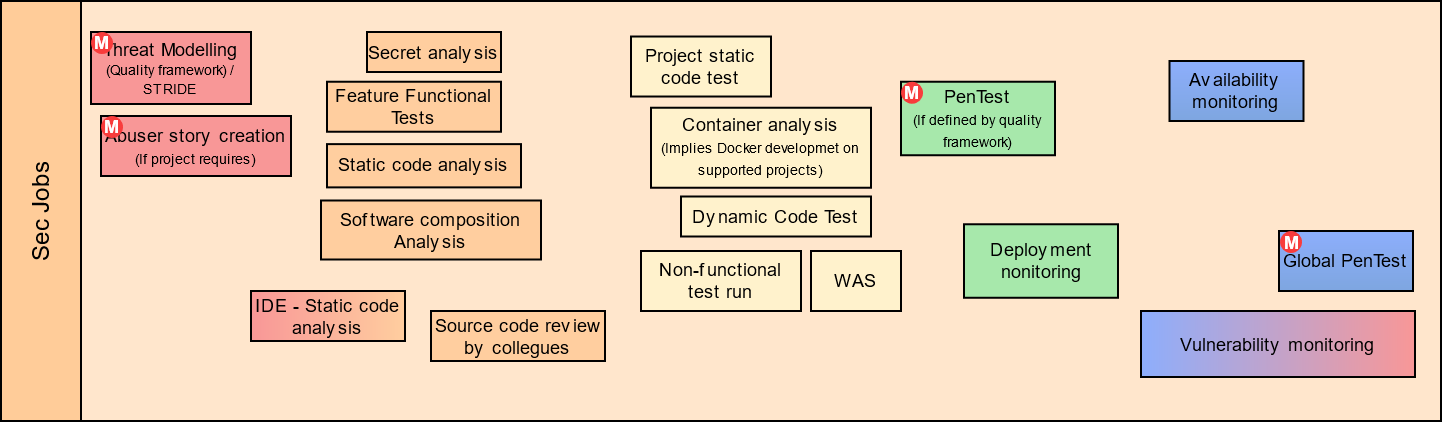
\includegraphics[width=\textwidth]{SDLC-Sec-SecJobs.png} 
  \label{fig:SDLCOverview-jobs}
\end{figure}

Cada una de estas tareas se traduce a un Topic.
Cada topic se compone en tickets.
A estos tickets, se les estima el tiempo que se va a dedicar en desarrollarlos.
Se hace este ejercicio por cada tarea que queremos llevar a cabo.
Al final, nos encontramos con una serie de topics, que debemos ordenar en cuando
a prioridades.

Por ejemplo, posiblemente, implementar una estrategia de
\href{https://docs.gitlab.com/ee/user/project/code_owners.html}{CODEOWNERS}
sea mas rápido que implementar una revision de código estático, pero si se ha
establecido mas prioritario lo segundo, entonces se posicionará antes en la lista de
tareas que debemos llevar a cabo.

Siguiendo con el ejemplo de los 
\href{https://docs.gitlab.com/ee/user/project/code_owners.html}{CODEOWNERS}:
Se segmenta la tarea ``Source code review by colleagues'' de la siguiente forma:

\begin{itemize}
  \item{\textbf{Topic:} ``Source code review by colleagues''}
    \subitem{\textbf{Ticket:} Research automated methods of ensuring source code
    review}
    \subitem{\textbf{Ticket:} Create \gls{PoC} demonstrating the solution}
    \subitem{\textbf{Ticket:} Implementation}
\end{itemize}

En este ultimo ticket, se describe la solución a la que se ha llegado en los dos
anteriores -- En este caso, seria usar
\href{https://docs.gitlab.com/ee/user/project/code_owners.html}{CODEOWNERS} --
y se divide en las fases que se estimen necesarias:

\begin{itemize}
  \item{Create groups}
  \item{Speak with \gls{HoT} to decide what files should be protected}
  \item{Map files to users}
  \item{Development of feature}
\end{itemize}

Una vez se desglosan las tareas, se calculan los tiempos iniciales (L0) que se
estima que duran.
Al acabar de estimar el tiempo de todas las tareas, se ordenan por prioridades y
se crea una estrategia de desarrollo a largo plazo.

\subsection{Estrategia a largo plazo de implementación del pipeline de
seguridad}

Aunque todas las herramientas y recomendaciones del ciclo de vida propuesto son
interesantes, cada una aporta ciertas características.
Dependiendo del estado de madurez de la organización en la que se va a implementar, 
es recomendable empezar por unas u otras herramientas y procesos.

En el estudio realizado por DORA y Google en enero de 2020, se ve claramente que
si se quiere llegar a mejorar el ``Software delivery and operational
performance'', entonces, se debe trabajar en areas como ``Change approvals'', o
``Lean product development'' entre otras (\cite{DORA2020}).

\begin{figure}[H]
  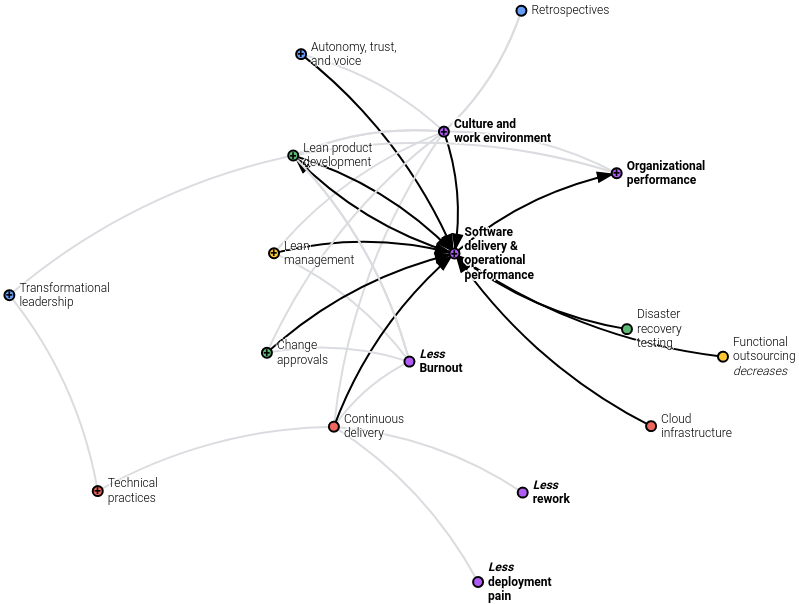
\includegraphics[width=\textwidth]{DORA-SDOP}
  \caption{Camino hacia una mejora en el despliegue de software y rendimiento
  operacional}
  \label{fig:DORA-SDOP}
\end{figure}

Este diagrama valida el esfuerzo que se esta haciendo en Scalefast por actualizar
el desarrollo de software para que siga un proceso mucho mas ágil.

Siguiendo con esta iniciativa, en el departamento de \gls{App-Sec}, se deben
priorizar las tareas a llevar a cabo.
Se ha decidido empezar por las tareas que menos tardan en implementarse pero que
mas repercusión tienen a la hora de mejorar el \gls{SDLC}.

Por este motivo, unas de las primeras tareas que se han seleccionado son la
revision de código fuente por compañeros de equipo, que finalmente se hará
estableciendo una política de 
\href{https://docs.gitlab.com/ee/user/project/code_owners.html}{CODEOWNERS} y
una herramienta para almacenar las credenciales de forma segura a lo largo de
todo el ciclo de vida del desarrollo de software.
Esta tarea usa \href{https://www.hashicorp.com/products/vault}{HASHICORP Vault}
como base de datos de los secretos de la aplicacion principal y pipeline que se
encarga de revisar el estado del despliegue.

Se han escocido estas dos tareas porque la primera añade directamente una
revision por parte de otro miembro de la organización, ademas, solo lo requiere
si es necesario, ya que si el archivo que se cambia no es critico, no se
requiere aprobación. Este proceso agiliza el desarrollo de software a la vez que
lo protege ante cambios indeseados a archivos críticos.
Por otro lado, se ha decidido usar
\href{https://www.hashicorp.com/products/vault}{HASHICORP Vault} 
porque asienta las bases de gestión de secretos para poder crear una estrategia
de despliegue de código en producción de forma automatizada y segura.

Al separar las tareas pendientes en una linea temporal, esta se prolonga hasta la
la segunda mitad de 2022.
%TODO: Seguir con las tareas: Añadir el listado de ellas y su distribución
%temporal

%TODO: Hablar de la organización de las tareas en quarters.

\subsection{Indicadores de éxito}

%TODO: Theory of constraints
%TODO: Value stream mapping

%Por que tomarlos
En los estudios se demuestra que las empresas lideres en el sector tienen una cultura
\gls{DevSecOps} madura. %TODO: Añadir una referencia a un estudio.
Estos estudios pueden servir para conseguir un voto de confianza por parte de los
responsables directivos pero para poder llevar a cabo el proyecto entero,
(sabiendo que tiene una estimación temporal mínima y que mantiene a todo el equipo
\gls{App-Sec} ocupado al menos hasta la segunda mitad de 2022) deben existir
datos propios, que justifiquen el esfuerzo que se esta realizando.
Una forma de justificar el esfuerzo, es mediante indicadores.

%Ventajas
La ventaja de estos indicadores, es que no solo sirven al \gls{c-level} para
tomar las decisiones estratégicas de la empresa sino que son útiles a toda la
parte técnica de la empresa.
Tanto los desarrolladores, \gls{DTL}, como los \gls{HoT} obtienen
información valiosa de estos indicadores y pueden medir y probar estrategias
contra un indicador o una medición base, construyendo así confianza explícita en
la estrategia que han tomado.
Esto proporciona a los equipos de desarrollo mucha agilidad.

%Ejemplos de indicadores
En el equipo de \gls{App-Sec}, los indicadores no son tan dinámicos como en el
equipo de desarrollo, debido a que la mayoría de las aplicaciones que se manejan
son preventivas, no reactivas.
Esto quiere decir que la mayor parte de las veces no partimos de una base sobre
la que medir, sino que se construye para que no sucedan problemas.
Aun así, algunos ejemplos de indicadores que sirven para ambos equipos pueden
ser el numero de errores que ha detectado la aplicacion de análisis estático de
código, el porcentaje de \gls{coverage} que tiene el código o el numero de
secretos que contiene el \gls{commit} candidato a producción.

% Como se miden?
Para medir la repercusión de los cambios implementados, \textbf{primero} se definen estos
indicadores, teniendo en cuenta que deben ser lo suficientemente generales como
para que no dependan de una tecnología, pero lo suficientemente específicos
como para que no se pierda su valor en posibles factores externos.
\textbf{Seguidamente} se miden, a poder ser, de forma automática el nivel base en el
que esta la plataforma en el momento de la medición.

%Cuando se miden
Estos indicadores deben medirse constantemente, o bien al pasar un periodo de
tiempo estipulado con anterioridad, o bien cuando se ha realizado un cambio que
afecta directamente estos indicadores.

%Herramientas que los midan
A medida que estos indicadores van madurando, se puede plantear crear una
plataforma que los mida de forma automática y cree un informe de las variaciones
de los indicadores que mas han fluctuado.

% Indicadores de éxito comunes
Los indicadores, cuando se usan en común con otras empresas, también pueden
servir para comparar la madurez de las mismas, en este caso en particular, de
los procesos \gls{DevSecOps}.
Algunos de los indicadores mas populares son:
El \textbf{``Lead time''}, esto es, el tiempo estimado desde que el código se ha subido
al control de versiones, hasta que ese mismo código se ha desplegado en
producción.
El \textbf{``Deploy frequency''}, mide la frecuencia con la que se despliegan
cambios al entorno de producción.
El \textbf{``Time to restore''} mide el tiempo que se tarda en restaurar el
servicio cuando ocurre algún contratiempo o incidente que afecta a los usuarios.
Por ultimo esta el \textbf{``Change fail percentage''}, que mide el porcentaje
de veces que se despliegan a producción cambios que desestabilizan la plataforma
y requieren acción.

%Que indicadores de éxito se han seleccionado?
Para medir el impacto de las dos tareas mencionadas anteriormente, se pueden
usar indicadores como el ``lead time'' o el ``numero de secretos en el entorno de
producción''.

%TODO: Seguir escribiendo por aquí

\chapter{Desarrollo de una tarea para el pipeline de seguridad}

A raíz del análisis de tareas pendientes para llegar al estado deseado del
\gls{pipeline}, se ha decidido que el primer desarrollo sea la implementación de
un mecanismo de gestión de secretos.
Esta decision estratégica cimienta la base para el nuevo enfoque hacia
\gls{DevSecOps} ya que desde el punto de vista de despliegue automatizado,
proporciona a los \gls{runner}s acceso a secretos, como las credenciales de
acceso al entorno de producción o las credenciales de la base de datos en
producción.
Ademas, tiene la capacidad de evitar que los desarrolladores guarden variables
en los propios archivos de código fuente, y tengan malas practicas de seguridad.
Tras haber comparado las distintas posibilidades, se ha decidido optar por usar
\href{https://www.hashicorp.com/products/vault}{HASHICORP Vault}.

\section{Securizacion de claves con HASHICORP Vault}

% Explicar como se ha llegado a HASHICORP Vault.
Durante la investigación realizada al inicio del proyecto, pudimos observar que
la plataforma por excelencia para Securizar las claves, tanto de la aplicación,
como de las herramientas que envuelven a la misma, como el \gls{pipeline} o los
\gls{runner}s que este emplea para llevar a cabo las tareas es 
\href{https://www.hashicorp.com/products/vault}{HASHICORP Vault}.
Esto es debido a que esta diseñada específicamente para cumplir este propósito.
Las alternativas a esta herramienta, suelen ser aplicaciones cuyo publico
objetivo son usuarios finales, por tanto estas herramientas se centran en la
simplicidad, la interfaz de usuario y la fácil curva de aprendizaje.
Aunque \href{https://www.hashicorp.com/products/vault}{HASHICORP Vault} no
cumpla con ninguna de estas características, tiene muy claras sus prioridades y
el uso que se va a hacer de la herramienta.

% Breve introducción de vault
\subsection{Casos de uso de HASHICORP Vault}

% Las ventajas que ofrece, frente a lo clásico
\subsection{Implementación de valores DevSecOps}

% La implementación.
\subsection{Implementación}

%     Creación de la VPC, con las sub-redes y las maquinas (Runner y EC2)

% Los resultados de la prueba de concepto

% La implementación de esa prueba de concepto a la realidad (Securizar pipelines
% de v3 web runner)

\chapter{Conclusiones}

\section{Indicadores de éxito}

\clearpage

\printglossary[type=\acronymtype]

\printglossary

%----------
%	Bibliography
%----------	

\clearpage
\addcontentsline{toc}{chapter}{Bibliografía}

\printbibliography


%---------- Appendix ----------	

% If your work includes Appendix, you can uncomment the following lines
%\chapter* {Appendix x} \pagenumbering{gobble} % Appendix pages are not numbered

\end{document}
